%%%%%%%%%%%%%%%%%%%%%%%%%%%%%%%%%%%%%%%%%%%%%%%%%%%%%%%%%%%%%%%%%%%%
%%%           Vorlage für eine Ausarbeitung an der DHBW          %%%
%%%                                                              %%%
%%%      Bereiche die bearbeitet werden müssen werden durch      %%%
%%%      einen solchen Kommentarblock eingeleitet und enden      %%%
%%%      mit der nächsten Trennlinie.                            %%%
%%%                                                              %%%
%%%      In dieser Datei müssen folgende Bereiche bearbeitet     %%%
%%%      werden:                                                 %%%
%%%      - Angaben zur Arbeit                                    %%%
%%%      - EIGENE KAPITEL EINFÜGEN                               %%%
%%%                                                              %%%
%%%      Benötigte Seiten und Verzeichnisse können unter         %%%
%%%      "Einführung und Verzeichnisse" ein- bzw. auskommentiert %%%
%%%      werden.                                                 %%%
%%%                                                              %%%
%%%%%%%%%%%%%%%%%%%%%%%%%%%%%%%%%%%%%%%%%%%%%%%%%%%%%%%%%%%%%%%%%%%%

\documentclass[a4paper,12pt]{article}
\usepackage[left=2.5cm,right=2.5cm,top=2.5cm,bottom=2.5cm,includehead]{geometry}      % Einstellungen der Seitenränder
\usepackage[english, ngerman]{babel}                                                  % deutsche Silbentrennung
\usepackage[utf8]{inputenc}                                                           % Umlaute
\usepackage[T1]{fontenc}                                                              % Umlaute auch richtig ausgeben
%\usepackage{newtxtext,newtxmath}                                                      % Font = Times New Roman
\usepackage{times}                                                      % Font = Times New Roman
\usepackage{hyperref}
\usepackage[nottoc]{tocbibind}
\usepackage{fancyhdr}
\usepackage{setspace}
\usepackage[backend=bibtex, citestyle=authoryear, bibstyle=authoryear]{biblatex}      % Bibliothek für Zitate
\usepackage{csquotes}                                                                 % Zusatzpacket für Zitate
\usepackage{amsmath}                                                                  % Zurücksetzen der Tabellen- und Abbildungsnummerierung je Sektion
\usepackage[labelfont=bf,aboveskip=1mm]{caption}                                      % Bild- und Tabellenunterschrift (fett)
\usepackage[bottom,multiple,hang,marginal]{footmisc}                                  % Fußnoten [Ausrichtung unten, Trennung durch Seperator bei mehreren Fußnoten]
\usepackage{graphicx}
\graphicspath{{./images/}}                                                            % Grafiken
\usepackage[dvipsnames]{xcolor}                                                       % Farbige Buchstaben
\usepackage{wrapfig}                                                                  % Bilder in Text integrieren
\usepackage{enumitem}                                                                 % Befehl setlist (Zeilenabstand für itemize Umgebung auf 1 setzen)
\usepackage{listings}                                                                 % Quelltexte
\usepackage{tabularx}                                                                 % Tabellen
\usepackage[addtotoc]{abstract}                                                       % Abstract
\usepackage[nohyperlinks, printonlyused, withpage]{acronym}                           % Abkürzungen

%%%%%%%%%%%%%%%%%%%%%%%%%%%%%%%%%%%%%%%%%%%%%%%%%%%%%%%%%%%%%%%%%%%%
%%%                      Angaben zur Arbeit                      %%%
%%%%%%%%%%%%%%%%%%%%%%%%%%%%%%%%%%%%%%%%%%%%%%%%%%%%%%%%%%%%%%%%%%%%
\newcommand{\vFirmenlogoPfad}{}                        %% relativer Pfad Bsp.: images/Firmenlogo.png
\newcommand{\vDHBWLogoPfad}{images/DHBW_logo.jpg}                          %% relativer Pfad Bsp.: images/DHBW_logo.jpg

\newcommand{\vTitel}{Prüfungsaufgabe im Modul Medientechnik und Usability}                           %%
\newcommand{\vUntertitel}{Gruppenspezifische Aufgabe}                      %%
\newcommand{\vArbeitstyp}{Hausarbeit}                      %% Projektarbeit/Seminararbeit/Bachelorarbeit
\newcommand{\vArbeitsbezeichnung}{Prüfungsaufgabe}              %% T1000/T2000/T3000

\newcommand{\vAutor}{Tobias Goetz - 4143507\\Philip Kuest - 3655862\\Noel Kempter - 2478267\\Marius Frick - 4387689}                           %% Vorname Nachname
\newcommand{\vMatrikelnummer}{}                  %% 7-stellige Zahl
\newcommand{\vKursKuerzel}{TIM21}                     %% Bsp.: TIT20
\newcommand{\vPhasenbezeichnung}{Theoriephase}               %% Praxisphase/Theoriephase
\newcommand{\vStudienJahr}{erste}                     %% erste/zweite/dritte
\newcommand{\vDHBWStandort}{Ravensburg}                    %% Bsp.: Ravensburg
\newcommand{\vDHBWCampus}{Friedrichshafen}                      %% Bsp.: Friedrichshafen
\newcommand{\vFakultaet}{Technik}                       %% Technik/Wirtschaft
\newcommand{\vStudiengang}{Informatik}                     %% Informationstechnik/...

\newcommand{\vBetrieb}{}                         %%
\newcommand{\vBearbeitungsort}{Friedrichshafen}                 %%
\newcommand{\vAbteilung}{}                       %%
\newcommand{\vBetreuer}{}                        %% Vorname Nachname

\newcommand{\vAbgabedatum}{\today}               %% DD. MONTH YYYY
\newcommand{\vBearbeitungszeitraum}{21.06.2022 - 26.07.2022}            %% DD.MM.YYYY - DD.MM.YYYY


%%%%%%%%%%%%%%%%%%%%%%%%% Eigene Kommandos %%%%%%%%%%%%%%%%%%%%%%%%%
% Definition von \gqq{}: Text in Anführungszeichen
\newcommand{\gqq}[1]{\glqq #1\grqq}


%%%%%%%%%%%%%%%%%%%% Zitatbibliothek einbinden %%%%%%%%%%%%%%%%%%%%%
\addbibresource{literatur/literatur.bib}
\addbibresource{literatur/literatur_usability.bib}
\addbibresource{literatur/literature-qwant.bib}
\addbibresource{literatur/literatur_googlestrategy.bib}


%%%%%%%%%%%%%%%%%%%%%%%% PDF-Einstellungen %%%%%%%%%%%%%%%%%%%%%%%%%
\hypersetup{
    bookmarksopen=false,
    bookmarksnumbered=true,
    bookmarksopenlevel=0,
    pdftitle=\vTitel,
    pdfsubject=\vTitel,
    pdfauthor=\vAutor,
    pdfborder={0 0 0},
    pdfstartview=Fit,
    pdfpagelayout=SinglePage
}


%%%%%%%%%%%%%%%%%%%%%%%% Kopf- und Fußzeile %%%%%%%%%%%%%%%%%%%%%%%%
\pagestyle{fancy}
\setlength{\headheight}{15pt}
\fancyhf{}
\fancyhead[R]{\thepage}


%%%%%%%%%%%%%%%%%%%%%%%%%%%%%% Layout %%%%%%%%%%%%%%%%%%%%%%%%%%%%%%
\onehalfspacing
\setlist{noitemsep}

\addto\catpionsngerman{
    \renewcommand{\figurename}{Abb.}
    \renewcommand{\tablename}{Tab.}
}
\numberwithin{table}{section}                               % Tabellennummerierung je Sektion zurücksetzen
\numberwithin{figure}{section}                              % Abbildungsnummerierung je Sektion zurücksetzen
\renewcommand{\thetable}{\arabic{section}.\arabic{table}}   % Tabellennummerierung mit Section
\renewcommand{\thefigure}{\arabic{section}.\arabic{figure}} % Abbildungsnummerierung mit Section
\renewcommand{\thefootnote}{\arabic{footnote}}              % Sektionsbezeichnung von Fußnoten entfernen

\renewcommand{\multfootsep}{, }                             % Mehrere Fußnoten durch ", " trennen


%%%%%%%%%%%%%%%%%%%%%%%%%%%%% Dokument %%%%%%%%%%%%%%%%%%%%%%%%%%%%%

\begin{document}


    %%%%%%%%%%%%%%%%%%% Einführung und Verzeichnisse %%%%%%%%%%%%%%%%%%%
    \pagenumbering{Roman}

    \begin{titlepage}
    \begin{minipage}{6in}
        \vspace*{-2cm}
        \centering
        \hspace{-2cm}
%        \ifx\vFirmenlogoPfad\empty
%        \else
%        \raisebox{-0.5\height}{\includegraphics[height=4cm]{\vFirmenlogoPfad}}
%        \fi
        \hfill
        \ifx\vDHBWLogoPfad\empty
        \else
        \raisebox{-0.5\height}{\includegraphics[height=4cm]{\vDHBWLogoPfad}}
        \fi
    \end{minipage}
    \begin{center}
        \vspace*{0.5cm}
        \Huge\textbf{\vTitel}\\
        \ifx\vUntertitel\empty
        \else
        \Large\textrm{\vUntertitel}\\
        \fi
        \vspace*{2cm}
        \Large\textbf{\vArbeitstyp}
        \ifx\vArbeitsbezeichnung\empty
        \else
        \textbf{\vArbeitsbezeichnung}
        \fi
        \\
        \normalsize
%        über die \vPhasenbezeichnung\ des \vStudienJahr{n}\ Studienjahrs \\
%        \vspace*{1cm}
        an der Fakultät für \vFakultaet\\
        im Studiengang \vStudiengang\\
        \vspace*{0.5cm}
        an der DHBW \vDHBWStandort\\
        \ifx\vDHBWCampus\empty
        \else
        Campus \vDHBWCampus\\
        \fi
        \vspace*{0.5cm}
        von\\
        \ifx\vAutor\empty
        \else
        \vAutor\\
        \fi
        \vspace*{1cm}
        \vAbgabedatum
        \vfill
    \end{center}
    \begin{tabular}{ll}
        Bearbeitungszeitraum:          & \vBearbeitungszeitraum          \\
%        Matrikelnummer, Kurs:          & \vMatrikelnummer, \vKursKuerzel \\
%        Dualer Partner:               & \vBetrieb                       \\
%        Betreuer des Dualen Partners: & \vBetreuer                      \\
    \end{tabular}
\end{titlepage}
\newpage
\setcounter{page}{2}
    % \thispagestyle{empty}
\section*{\Huge{Sperrvermerk}}

\addcontentsline{toc}{section}{Sperrvermerk}
gemäß Ziffer 1.1.13 der Anlage 1 zu §§ 3, 4 und 5  der Studien- und Prüfungsordnung für die Bachelorstudiengänge im Studienbereich Technik der Dualen Hochschule Baden-Würt­tem­berg vom 29.09.2017.\\

\noindent \gqq{Der Inhalt dieser Arbeit darf weder als Ganzes noch in Auszügen Personen außerhalb des Prüfungsprozesses und des Evaluationsverfahrens zugänglich gemacht werden, sofern keine anders lautende Genehmigung vom Dualen Partner vorliegt.}

\vfill
\leavevmode
\newline
\parbox{6cm}{\centering \vBearbeitungsort, \vAbgabedatum\hrule\strut\centering\footnotesize Ort, Datum} 
\hfill
\parbox{6cm}{\hspace{1pt} \vAbteilung\hrule\strut\centering\footnotesize Abteilung, Unterschrift}

\newpage
    \thispagestyle{empty}
\section*{\Huge{Selbstständigkeitserklärung}}

\addcontentsline{toc}{section}{Selbstständigkeitserklärung}
gemäß Ziffer 1.1.13 der Anlage 1 zu §§ 3, 4 und 5  der Studien- und Prüfungsordnung für die Bachelorstudiengänge im Studienbereich Technik der Dualen Hochschule Baden-Würt­tem­berg vom 29.09.2017.

\noindent Ich versichere hiermit, dass ich meine Bachelorarbeit ( bzw.\ Projektarbeit oder Studienarbeit bzw.\ Hausarbeit ) mit dem Thema:
\begin{center}
	\Large\textbf{\vTitel}
\end{center}
selbstständig verfasst und keine anderen als die angegebenen Quellen und Hilfsmittel benutzt habe.
Ich versichere zudem, dass die eingereichte elektronische Fassung mit der gedruckten Fassung übereinstimmt.

\vfill
\leavevmode
\newline
\parbox{6cm}{\centering \vBearbeitungsort, \vAbgabedatum\hrule\strut\centering\footnotesize Ort, Datum} 
\hfill
\parbox{6cm}{\hspace{1pt} \vAbteilung\hrule\strut\centering\footnotesize Abteilung, Unterschrift}

\newpage
    \phantomsection
\newenvironment{keywords}{
	\begin{flushleft}
	\small	
	\textbf{
		\iflanguage{ngerman}{Schlüsselwörter}{\iflanguage{english}{Keywords}{}}
	}
}{\end{flushleft}}

% Deutsche Zusammenfassung
\begin{abstract}
	Das Internet ist aus dem modernen Leben kaum mehr wegzudenken und damit gilt das Selbe für Suchmaschinen wie
	Google, Bing und Co welche das durchforsten des Internets überhaupt erst ermöglichen.
	Um sich die Gunst der Nutzer zu erkämpfen und die stärkste Position in diesem Markt einzunehmen haben sich Suchmaschinen
	stetig weiter entwickelt um den Konkurrenten stets einen Schritt voraus zu sein.

	Ziel dieser Arbeit ist es einen kurzen Überblick über die Geschichte von Suchmaschinen und im Speziellen den Werdegang
	von Google zur meist genutzten Suchmaschine der Welt zu geben, sowie einen eher unbekannten Konkurrenten des
	Internetgiganten zu betrachten und einen kleinen Ausblick auf die potentielle Zukunft von Suchmaschinen zu geben.

	Um dieses Ziel zu erreichen werden in dieser Arbeit die Ergebnisse von einer im Rahmen dieses Projekts durchgeführten
	Konkurrenzanalyse sowie eines Usability-Tests mit Google, Bing und Qwant als betrachteten Zielen dargelegt.
	
\end{abstract}

% Schlüsselwörter Deutsch
\begin{keywords}

\end{keywords}


\selectlanguage{english}
% Englisches Abstract
\begin{abstract}
	To imagine a modern world without the internet is nearly impossible today and therefore the same also goes for search
	engines like Google, Bing and others since they make it even possible to traverse the internet.
	In order to attract the most users and to gain the most influential position in this market search engines have
	constantly evolved in order to always be one step ahead of their competitors.

	The aim of the presented work is to give a brief summary of the history of search engines and in particular how
	Google became the most used search engine in the world, as wall as look at a rather less known competitor of the
	internet giant and give a small glimpse of the potential future of search engines.

	In order to do so the presented work will showcase the results of a competitor analysis as well as a usability test
	with Google, Bing and Qwant as their targets, that were conducted as part of this project.
\end{abstract}

% Schlüsselwörter Englisch
\begin{keywords}

\end{keywords}


\selectlanguage{ngerman}
\newpage
    \tableofcontents
\newpage
    \section*{Abkürzungsverzeichnis}
\addcontentsline{toc}{section}{Abkürzungsverzeichnis}
\begin{acronym}
  \acro{DHBW}[DHBW]{Duale Hochschule Ba\-den-\-Würt\-tem\-berg}
  \acroplural{DHBW}[DHBW]{Dualen Hochschule Ba\-den-\-Würt\-tem\-berg}

  \acro{WCAG}[WCAG]{Web Content Accessibility Guidelines}
\end{acronym}
\newpage
    \listoffigures
\newpage
    \listoftables
\newpage
    % \section*{Vorwort}
\addcontentsline{toc}{section}{Vorwort}
\newpage


    %%%%%%%%%%%%%%%%%%%%%%%%%%%%% Kapitel %%%%%%%%%%%%%%%%%%%%%%%%%%%%%%
    \pagestyle{fancy}
    \fancyhead[L]{\nouppercase{\rightmark}}    % Abschnittsname im Header
    \pagenumbering{arabic}

    %%%%%%%%%%%%%%%%%%%%%%%%%%%%%%%%%%%%%%%%%%%%%%%%%%%%%%%%%%%%%%%%%%%%
    %%%%                   EIGENE KAPITEL EINFÜGEN                  %%%%
    %%%%%%%%%%%%%%%%%%%%%%%%%%%%%%%%%%%%%%%%%%%%%%%%%%%%%%%%%%%%%%%%%%%%
    \section{Einleitung}\label{sec:einleitung}
Wie kann Google den Markt der Suchmaschinen mit über 90 Prozent Marktanteil so stark dominieren und welche Konkurrenz gibt es?
Wäre baldiger Wechsel an der Spitze des Marktes denkbar?
In der folgenden Arbeit soll der Markt der Suchmaschinen und einzeln ausgewählte Vertreter analysiert werden.
Um die Situation auf dem Markt zu verstehen und die wichtigsten Punkte kennenzulernen, in denen sich eine Suchmaschine beweisen muss,
wird im Folgenden zuerst eine Konkurrenzanalyse durchgeführt, bei der zum einen der \("\)big-player\("\) Google,
aber auch der Konkurrent Bing und eine Start-up-Suchmaschine namens Qwant betrachtet werden.
Um die Konkurrenzsituation genau zu erläutern werden hier verschiedene Aspekte der Suchmaschinen untersucht, analysiert und dann einander gegenüber gestellt.
Fortlaufend wird im zweiten Kapitel herausgearbeitet wie Google schon früh aus der Menge der Suchmaschinen herausstach und den Markt bis heute dominiert.
Hierbei wird Googles Strategie zu unterschiedlichen Zeitpunkten bewertet und untersucht, wie sie auf die heutige Topposition der Suchmaschine einwirkten.
Vom \("\)big-player\("\) zu einer bisher ziemlich kleinen, unbekannten Suchmaschine,
wird dann das französische Start-up Qwant betrachtet, wessen Suchmaschine sich trotz eines bisher kleinen Marktanteils großer Beliebtheit erfreut.
Dabei werden die Gründe für den Erfolg von Qwant, seine Chancen und Vorteile gegenüber der bereits genannten Konkurrenz herausgearbeitet.
Ein wichtiger Aspekt für Suchmaschinen ist ihre Finanzierung, da diese oft gar nicht so offensichtlich ist.
Folgend werden im vierten Kapitel die verschiedenen Finanzierungskonzepte und ihre Rolle in der Aufstellung am Markt untersucht.
Um die praktische Erfahrung mit den Suchmaschinen Google, Bing und Qwant herauszuarbeiten werden im Anschluss die Ergebnisse von Usability-Tests mit den drei Anbietern präsentiert.
Diese sollen die Anwendung der Suchmaschinen im Alltag analysieren und so weitere Aspekte, Vor- und Nachteile einzelner Anbieter aufzeigen.
Zuletzt wird betrachtet, wie Suchmaschinen, vor allem Google, uns als Nutzer beeinflusst oder schon beeinflusst hat.
Auch soll hier ein Blick in die Zukunft geworfen werden und betrachtet werden, wie Google und Co uns weiter beeinflussen könnten und welche Rolle sie in der Zukunft spielen könnten.
    \section{Konkurrenzanalyse}\label{sec:konkurrenzanalyse}
Diese Arbeit beginnt mit einer Konkurrenzanalyse der Webseiten www.google.com, www.bing.com sowie www.qwant.com.
Dabei wird insbesondere auf den Inhalt der jeweiligen Webseiten, die Zielgruppenorientierung, das Design, die Informations-
und Navigationsarchitektur, die Texte sowie auf die Technik der Seiten eingegangen. Zusätzlich zu diesen Punkten wird auch
auf die Qualität der Suchvorschläge eingegangen.

\subsection{Inhalt}\label{subsec:inhalt}
Das Ziel aller drei Webseiten ist es, den Nutzern die Möglichkeit zu bieten, das Internet nach Webseiten zu einem gewissen
Thema zu durchsuchen.
Ohne das Vorwissen, dass die drei Seiten dies anbieten, ist diese Dienstleistung allerdings nicht auf den ersten
Blick erkenntlich.
\begin{figure}[ht]
    \centering
    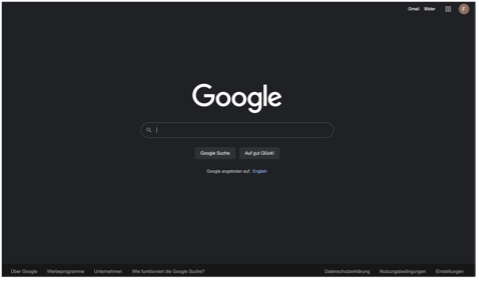
\includegraphics{Google Startseite}
    \caption{Startseite von Google}\label{fig:figure}
\end{figure}

Beispielsweise besteht die Startseite von Google nur aus einer Leiste, in der man etwas eingeben kann.
Ohne eine Anleitung, was sie in dieser Leiste eingeben können, führt dies am Anfang für Verwirrung. Nutzer, die mit Google
vertraut sind, profitieren allerdings von dieser Anordnung, da diese nicht von der Funktionalität ablenkt.
\begin{figure}[ht]
    \centering
    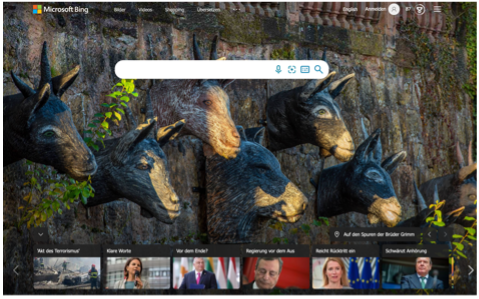
\includegraphics{Bing Startseite}
    \caption{Startseite von Bing}\label{fig:figure2}
\end{figure}
Einen ähnlichen
Aufbau bietet Microsoft mit ihrer Suchmaschine Bing. Hierbei werden standardmäßig allerdings noch aktuelle Nachrichten sowie
ein Hintergrundbild angezeigt.
\begin{figure}[ht]
    \centering
    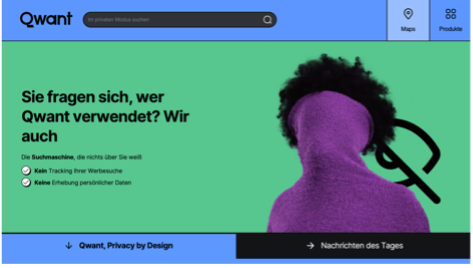
\includegraphics{Qwant Startseite}
    \caption{Startseite von Qwant}\label{fig:figure3}
\end{figure}
Einzig Qwant folgt diesem Schema nicht ganz.
Bei dieser Seite ist die Suchleiste, welche die
Hauptfunktion ist, im oberen Bereich, wodurch der Fokus auch auf die Texte in der Mitte des Bildschirms fallen kann.
Dies erschwert es Erstanwendern noch mehr als bei den Konkurrenten, die Funktion intuitiv zu bedienen.
Somit mangelt es allen Suchmaschinen an Selbstbeschreibungsfähigkeit.
Dies wäre nur gewährleistet, „wenn jeder einzelne Dialogschritt unmittelbar
verständlich ist“\autocite[Seite 6]{Maulhardt.20220506}.
Auch adäquate Anleitungen werden nicht zur Verfügung gestellt.

Trotz der oben genannten Kritik bieten alle drei Suchmaschinen, insbesondere für erfahrene Anwender, einen echten Mehrwert.
So erleichtern es alle Seiten, sich im Internet zurechtzufinden und ermöglichen das Finden bestimmter Webseiten.

\subsection{Zielgruppenorientierung}\label{subsec:zielgruppenorientierung}
Wie jedes Produkt haben auch diese drei Webseiten Zielgruppen, welche durch verschiedene Aspekte wie Design oder Inhalt
angesprochen werden sollen.
Diese Zielgruppen sollen nachfolgend herausgearbeitet werden und die Orientierung an diesen
bewertet werden.

Um herauszufinden, wie gut die drei Seiten ihre Zielgruppen abbilden, ist es zuerst nötig, diese Zielgruppen zu identifizieren.
Diese Adressaten haben bei allen drei Seiten eine große Schnittmenge, unterscheiden sich allerdings in Kleinigkeiten.
Da alle drei Unternehmen, welche die Suchmaschinen betreiben, einen möglichst großen Umsatz durch Werbeplatzierungen
erzielen wollen, versuchen diese, eine möglichst große Zahl an Usern zu generieren, weswegen die Seiten auch auf diesen Zweck zugeschnitten sind.
Da nicht alle Menschen Zugang zu Internet haben, richten sich die Webseiten, insbesondere an Personen mit diesem Zugang.
Ansonsten ist die Bandbreite an potenziellen Nutzergruppen sehr groß.
Dies erkennt man auch an der großen Auswahl an Sprachen, in welchen die Webseiten dargestellt werden können.
So bietet Google knapp 150 Sprachen an, Bing knapp 100.
Qwant müsste sich hingegen noch breiter aufstellen.
Mit gerade einmal 12 Sprachen wird eine große Zahl an
potenziellen Nutzern nicht angesprochen.

Eine Besonderheit gibt es bei der Zielgruppe von Qwant jedoch noch zu beachten.
Sie versuchen insbesondere Leute anzusprechen, denen Privatsphäre wichtig ist.
Dies wird bereits auf der Startseite klar.
Auf dieser wird damit geworben, dass die Suchmaschine
nichts über die Nutzer weiß, da diese keine persönlichen Daten erheben oder die Websuche tracken.

Ebenfalls spricht die Suchmaschine Qwant eine kindlichere Zielgruppe bzw. deren Eltern an.
In einem klar abgegrenzten Bereich wird es den Eltern ermöglicht, für die Kinder eine sichere Suche im Internet zu gewährleisten.
Bei den Konkurrenten fehlt ein solches Angebot.

\subsection{Design}\label{subsec:design}
Ein wichtiger Punkt einer Webseite ist dessen Design.
„Unser visuelles System ist darauf ausgelegt, schnell zu entscheiden, ob wir etwas gut oder schlecht finden.
Dabei wird der Ersteindruck einer Website vor allem durch die Schönheit,
also die visuelle Ästhetik, bestimmt.“\autocite[Seite 43]{Thielsch.}.
Somit ist das Design eines der zentralen Elemente, welches besonders gut ausgearbeitet sein muss.
Dabei gehen alle drei Suchmaschinen einen anderen Weg.

Googles Auftritt ist sehr minimalistisch gehalten.
Bis auf ein Logo, welches sich in unregelmäßigen Zeitabständen verändert,
ist nur die Suchleiste in der Bildmitte zu sehen.
Der Hintergrund ist dabei je nach Einstellung des Dark-Modes dunkelgrau oder weiß.
Diese fehlende Farbauswahl spiegelt nicht direkt das Firmenimage von Google wider, welches, wie am farbenfrohen
Firmenlogo zu erkennen, eher verspielt, modern und innovativ wirkt.
\begin{figure}[ht]
    \centering
    
\includegraphics[width=0.3\linewidth]{Google Firmenlogo}
    \caption{Firmenlogo von Google\autocite{.2020}}\label{fig:figure4}
\end{figure}

Im Gegensatz zu diesem einfarbigen Design von Google bietet Bing die Möglichkeit ein Landschaftsbild als Hintergrund zu
setzen, welches sich täglich ändert.
Diese Veränderung bringt regelmäßige Abwechslung, was auf den Nutzer erfrischend wirken kann.
Außerdem wirken die Bilder freundlich auf die Nutzer, weswegen die Startseite von Bing, gegenüber der von Google,
bevorzugt werden könnte.
\begin{figure}[ht]
    \centering
    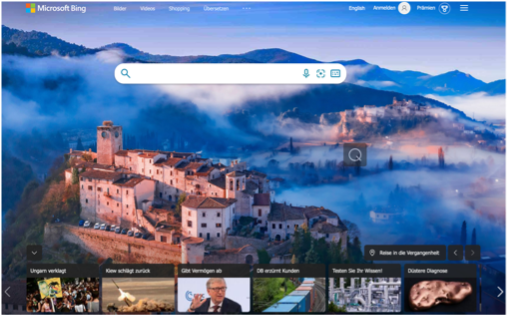
\includegraphics{Bing Startseite 2}
    \caption{Design der Startseite von Bing}\label{fig:figure5}
\end{figure}

Am auffälligsten und damit auch am meisten Raum für Analyse bietend ist allerdings die Startseite von Qwant. Mehrere
klassische Formen des Kontrasts wurden hier benutzt.
Zum einen ist der starke Kontrast zwischen gelb und blau auffällig.
\begin{figure}[ht]
    \centering
    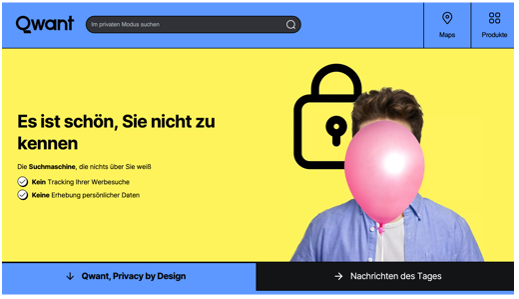
\includegraphics{Qwant Startseite Design}
    \caption{Design der Startseite von Qwant}\label{fig:figure6}
\end{figure}
Dies erinnert stark an einen Komplementärkontrast.
Dies bedeutet, dass sich die beiden Farben im Farbenkreis gegenüberliegen\autocite[Seite 33]{Maulhardt.20220513}.
Bei Betrachtung des Farbkreises nach Itten (\ref{fig:farbkreis}) fällt dies ebenfalls auf.
Auch ein Warm-Kalt-Kontrast ist vorhanden. Hierbei wird die warme Farbe Gelb der kalten Farbe Blau direkt gegenübergestellt\autocite[Seite 34]{Maulhardt.20220513}.
Zuletzt beinhaltet die Startseite noch einen Farbe-an-sich-Kontrast.
\begin{figure}[ht]
    \centering
    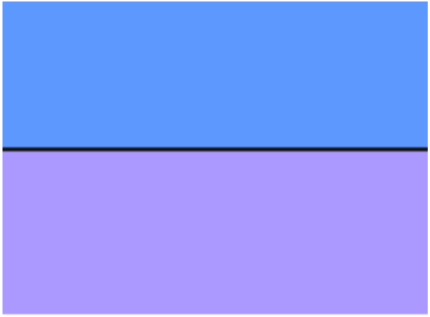
\includegraphics{Qwant Startseite 3}
    \caption{Startseite von Qwant}
    \label{fig:qwantstartseite3}
\end{figure}
Dieser ergibt sich dadurch,
dass wie bei Abbildung~\ref{fig:qwantstartseite3} die Grundfarben Blau und Lila gegenübergestellt werden\autocite[Seite 38]{Maulhardt.20220513}.
All diese Kontraste lassen die Startseite von Qwant lebendig wirken, was mit dem Image der Firma bzw.\ der Suchmaschine übereinstimmt.
Trotzdem wäre es wünschenswert, wenn das Erscheinungsbild angepasst werden könnte, da dies einigen aufgrund der starken
Kontraste abschrecken könnte.
Diese junge Zielgruppe ist auch aufgrund der Benutzung von Emojis in beispielsweise den
Filtereinstellungen erkennbar.

Positiv fällt bei allen drei Seiten auf, dass diese einen einstellbaren Dark Mode besitzen, welcher es ermöglicht, das Design zu verändern.
Zusätzlich bietet Bing die Möglichkeit das oben angesprochene Hintergrundbild nicht anzeigen zu lassen,
sodass die Optik mit entweder dunkelgrau oder weiß als Hintergrund sehr stark Google ähnelt.

\subsection{Informations- und Navigationsarchitektur}\label{subsec:informations--und-navigationsarchitektur}
Die Navigationsarchitektur ist auf allen drei Seiten relativ gleich aufgebaut.
Die Startseite besteht dabei aus einer Suchleiste,
welche nach der Suche an den oberen Bildrand geht, wobei die vorgeschlagenen Webseiten darunter angezeigt werden.
Das Logo der Suchmaschine dient dabei immer als Homebutton.
Diese Grundstruktur ist für Personen, die die Funktionalität der
Seiten kennen sehr einfach zu durchschauen, da sie sich von Anbieter zu Anbieter nicht verändert.
Allerdings unterscheidet sich die Architektur in Kleinigkeiten.
Darauf wird im Nachfolgenden eingegangen.

Google bietet in der rechten oberen Ecke die Möglichkeit, den Account zu managen, auf zahlreiche andere Google Dienste zu
wechseln oder eine Bilder\-Suche durchzuführen.
Am unteren Bildrand wird zum einen auf Informationsseiten zu Google verwiesen,
wie auch die Möglichkeiten geboten, die Einstellungen zu ändern.
Diese Auswahlmöglichkeiten sind allerdings sehr klein gehalten,
wodurch sie für Leute, welche nicht mehr so gut sehen können, nicht mehr gut erkennbar sind.
Auch ein geringer Kontrast erschwert die Lesbarkeit dieser Elemente.

Bing hat im Gegensatz zu Google ein paar Punkte, welche positiv aufgefallen sind.
Insbesondere die Möglichkeit, sich Newsartikel sich anzeigen zu lassen,
auf welche man bei Bedarf klicken kann, stach dabei im direkten Vergleich heraus.
Ein weiterer Punkt ist die Verwendung von Icons, welche bei Google nur sehr wenig eingesetzt werden.
Dahingegen schafft es Bing, diese gezielt und unterstützend zu normalem Test einzusetzen, was die Bedienung vereinfacht.
\begin{figure}[ht]
    \centering
    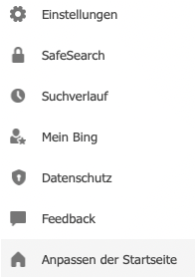
\includegraphics{Bing Icons 1}
    \caption{Icons von Bing}\label{fig:figure8}
\end{figure}
Diese Icons sind dabei auch gemäß den Regeln
für die Gestaltung einer Navigationsleiste\autocite[Seite 17]{Maulhardt.20220621b} selbsterklärend, da sie alle standardmäßig auch von
anderen Webseiten für dieselben Funktionen verwendet werden.

Zuletzt wird die Navigationsstruktur von Qwant analysiert.
Diese hat sowohl Vor- als auch Nachteile gegenüber den Konkurrenten.
Zum einen ist die Zahl an Auswahlpunkten, zumindest wenn auf der Startseite nicht gescrollt wird, sehr leicht überschaubar.
So kann man nur zwischen Maps, den Produkten, Informationen über Qwant und den Nachrichten des Tages wählen.
Diese geringe Zahl ermöglicht es, vor allem im Vergleich zu den Konkurrenten,
welche 13 (Google) und 9 (Bing) Auswahlpunkte direkt auf der
Startseite haben, schnell einen Überblick über die Struktur der Seite zu erlangen.
Damit halten sich die beiden Seiten auch nicht an die Regel,
dass nur maximal sieben Buttons gleichzeitig zu sehen sind, da das Gehirn nicht mehr auf einen Blick
wahrnehmen kann\autocite[Seite 16]{Maulhardt.20220621b}.
Negativ wiederum an der Startseite von Qwant ist, dass der Punkt „Maps“, welcher
in Abbildung~\ref{fig:qwantnavigation} zu sehen ist, sich mit dem Menü, welches unter Produkte gezeigt wird, überschneidet.
\begin{figure}[h]
    \centering
    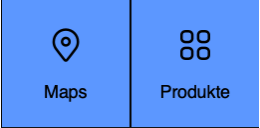
\includegraphics{Qwant Navigation}
    \caption{Navigation von Qwant}
    \label{fig:qwantnavigation}
\end{figure}

So werden dabei die
Produkte Search und Maps vorgeschlagen, obwohl man auf Search bereits ist und Maps einfacher über den extra Button Maps aufrufbar ist.
Einzig das Produkt „Junior“ ist in dieser Reihe neu.
Ebenso negativ anzumerken ist, dass die Einstellungen schwer zu finden sind.
So muss der Nutzer bis ganz nach unten scrollen, damit sehr klein unten rechts der Button Einstellungen zu sehen ist.
Dieser ist zusätzlich nicht einmal deutlich hervorgehoben und wird mit grauer Schrift auf schwarezm Hintergrund dargestellt.

\subsection{Text}
Aufgrund der Ziele der Webseitenbetreiber sind die Seiten mit wenig Text versehen. Stattdessen ist der Aufbau der Seiten
so gestaltet, dass der Nutzer sich intuitiv zurechtfindet. Außerdem ist es nicht das Ziel der Suchmaschinen den User durch
lange Texte vom eigentlichen Sinn der Seite abzulenken, nämlich dem Suchen nach anderen Webseiten. Einzig Qwant fällt aus
diesem Muster heraus.
\begin{figure}[ht]
    \centering
    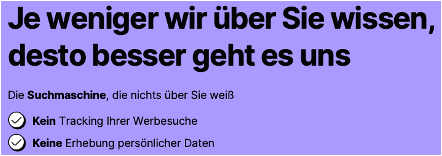
\includegraphics{Qwant Texte}
    \caption{Texte von Qwant}\label{fig:figure9}
\end{figure}

Sie versuchen den Besucher auf der Homepage von ihrem Konzept der privaten Suche mit der Hilfe von
Text zu überzeugen. Dabei befolgen Sie auch alle Regeln der Textgestaltung\autocite[Seite 5ff]{Maulhardt.20220621b}. Durch kurze prägnante Texte,
in welchen durch fette Schrift das wichtigste markiert ist, wird die Kernaussage gut dargestellt.

\subsection{Technik}
Ebenso wichtig wie die bisher angesprochenen Analysekriterien ist die Technik, mit welcher die Webseiten gestaltet wurden.
So können beispielsweise lange Ladezeiten dafür sorgen, dass der Nutzer eine andere Suchmaschine in Zukunft benutzen wird.
Um diese Technik möglichst objektiv bewerten zu können wurde ein standardisierter Test durchgeführt, welcher Webseiten nach
vier Analysekriterien beurteilt. Dieser Test namens „Lighthouse“ ist dabei eine Chrome-Erweiterung. Die genauen Ergbeniss
sind im Anhang zu finden.

Google schneidet dabei am besten ab. Nur im Bereich SEO, was für Search Engine Optimization steht, ist noch wirkliches
Potenzial, die Seite zu verbessern. Ansonsten ist Google in den drei Bereichen Performance Accessibility und Best Practices
in einem sehr guten Bereich. Insbesondere die Performance, welche bei den anderen beiden Anbietern schlechter ist,
sticht dabei heraus.

Bing hingegen hat insbesondere im Bereich Performance noch Verbesserungsbedarf. Hierbei wird empfohlen, ungenutzten JavaScript
Code zu reduzieren. Ebenso könnte der Analysepunkt Accessibility besser sein.

Qwant schneidet im Bereich Performance mit gerade einmal 54 von 100 möglichen Punkten am schlechtesten ab. Dabei wird ebenfalls
geraten, ungenutzten JavaScript Code zu reduzieren.

\subsection{Qualität der Suchvorschläge}
Bei der Analyse einer Suchmaschine sind auch die Suchvorschläge sowie die Ergebnisse zu evaluieren. Dies wurde exemplarisch
an dem Begriff Medientechnik untersucht. Google und Bing sind dabei auf einem vergleichbaren Niveau. Beide Suchmaschinen
bieten zahlreiche Möglichkeiten zum bisher eingegebenen Begriff „Mediente“, wie beispielsweise „Medientechnik“ oder „Medientechnologe".

Ebenso werden zahlreiche verschiedene Informationen nach der Suche präsentiert, welche über die reine Auflistung von Webseiten hinausgehen.
So boten beide Webseiten Unternehmen in der Nähe des Benutzers an.
Bing präsentierte zusätzlich Videos, wohingegen Google auf den Wikipedia Artikel zu Medientechnik verwies.

Dahingegen bot Qwant keine Vervollständigung des Begriffs „Mediente“ an. Ebenso besteht Verbesserungsbedarf in der Präsentation
der Webseiten. In diesem Fall wurden nur mögliche Webseiten aufgelistet, während beispielsweise Google
interaktive Schaltflächen zu Maps und Wikipedia anbot.
    %! Author = noel.kempter
%! Date = 24.07.2022

\section{Google-Strategie}\label{sec:google-strategie}

In diesem Kapitel werfen wir einen kurzen Blick auf die Geschichte von Suchmaschinen und im Speziellen den Werdegang
von Google zur, mit Abstand, meist verwendeten Suchmaschine der Welt und der Strategie die das ermöglichte.

\subsection{Geschichte}\label{subsec:geschichte}
Die Geschichte der Suchmaschinen beginnt mit der Entstehung des Internets selbst Anfang der 90er Jahre.
Schon damals gab es unter den Suchmaschinen klare Favoriten, doch keiner davon hieß Google.
Die ersten großen Kompetitoren waren die Suchmaschinen AskJeeves, Lycos und Alta Vista, von denen heute keine mehr
Bestand als normale Suchmaschine hat.
Auch BackRub, entwickelt 1995 von den Google-Gründern Larry Page und Sergey Brin und daher von vielen als Vorgänger von
Google bezeichnet, konnte früh überzeugen hatte jedoch noch lange nicht solch eine dominante Marktstellung wie heute.
Wenig später kamen die auch heute noch relevanten Suchmaschinen Yahoo und MSN(2009 umbenannt in Bing) mit
ins Rennen.
Heute teilen sich Google, Yahoo und Bing je nach Region insgesamt bis zu 95\% der Marktanteile, wobei Google stets
mindestens ein 7-faches der Marktanteile aller Mitbewerber gemeinsam ausmacht.

\subsection{Google Strategie}\label{subsec:google-strategie}
Dazu kommen konnte es dank der außergewöhnlichen Unternehmensstrategie von Google, welche sich auf verschiedene Grundlagen
stützt.
Ein Aspekt des Erfolges von Google ist die Innovativität.
Schon in den Anfangstagen der Suchmaschine konnte diese durch innovatives Design und Ideen, welche zu schnelleren und
besseren Suchergebnissen führte überzeugen.
So war es Google welche mit dem PageRank zum ersten Mal eine Bewertungsskala für Webseiten anlegte und aktiv in die
Anzeige von Suchergebnissen mit einbezog.
Dieses Ranking-Schema bewerte Webseiten nicht nur anhand des Inhalts, sondern unter anderem auch an der Anzahl
eingehender Links einer Seite, der Qualität der Seiten von denen diese Links kommen, dem Layout beziehungsweise Design
der Seite bewertet nach W3C-Kriterien und vielen weiteren Faktoren.
Damit konnte Google schon Ende der 90er Jahre qualitativ hochwertigere Suchergebnisse liefern als alle Konkurrenten.
Ein weiterer Erfolgsaspekt ist das Design der Seite dem bis zum heutigen Tage treu geblieben wird.
Was heute als eher schlicht, teilweise schon langweilig, empfunden werden könnte hatte in den frühen Tagen des Internets
klare Vorteile, welche mit zum Sieg über die Mitbewerber beitrugen.
Denn während Bing, Yahoo und andere Konkurrenten ihre Seiten zu Webportalen weiterentwickelten, auf denen neben der
Suchmöglichkeit auch aktuelle Nachrichten, dass Wetter und weitere Informationen zu sehen waren, blieb Goggle dem schlichten
Design treu, was aufgrund der damals noch stark begrenzten Ressourcen in Sachen Rechenleistung und Internetgeschwindigkeit
zu deutlich schnelleren Ladezeiten als bei den Mitbewerbern und damit einer besseren User-Experience führte.
Außerdem konnte Google seinen Index, das heißt die Anzahl der bekannten und vernetzten Seiten schneller ausbauen als die
Konkurrenten und zur Jahrtausendwende mit über einer Milliarde bekannten Webdokumenten zur größten Suchmaschine der Welt.
Des Weiteren führte die Einführung von GoogleAdWords, einem Service welcher es Kunden ermöglicht ihre Werbung an
bestimmte Suchbegriffe zu koppeln und gemeinsam mit den eigentlichen Suchergebnissen anzeigen zu lassen, im Jahr 2000 und
der Börsengang im Jahr 2004 zu massiven Geldeinnahmen und dem Wunsch vieler an diesem Erfolg Teil zu haben.
Doch anstatt sich auf diesem Erfolg auszuruhen wurden diese Einnahmen verwendet, um die Marktpalette des Internetgiganten
zu erweitern, wodurch dieser den Konkurrenten abermals einen Schritt voraus war.
So wurden in den Jahren 2004/2005, dem Zeitraum in dem Google alle Konkurrenten endgültig zurückließ, die Dienste Google Mail,
Google Maps und Google Earth in Betrieb genommen.
Während es für die beiden letzteren Dienste aufgrund der Neuartigkeit dieser Technologien kaum ernst zu nehmende
Konkurrenz gab, war ein E-Mail-Service mitte der 2000er längst nichts Ungewöhnliches mehr.
Was Gmail jedoch auszeichnete und letzten Endes zum Erfolg verhalf, war die damalige Größe des Postfachs von einem
Gigabyte Speicher, welcher die Konkurrenten, deren Postfächer meist auf zwei bis höchstens zwanzig Megabyte beschränkt
waren, um das fünfzig- bis sogar fünfhundertfache übertrumpfte.
Auch durch das behutsam gepflegte Firmenimage gepaart mit Gags und Events um die Nutzer zu belustigen kann
die Suchmaschine überzeugen.
So kommt das auf der Startseite angezeigte Firmenlogo, wie in Abbildung ~\ref{fig:google_doodle} zu erkennen, je nach Anlass in
unterschiedlicher Aufmachung daher und auch Easter Eggs, das heißt versteckte Funktionen, die keinen wirklichen Sinn haben,
sind in der Suchmaschine verbaut(wer so etwas noch nicht kennt, muss in der Sucheingabe nur einmal \('\)do a barrel roll' eingeben)
und machen das Surfen zu einer waren Experience.
Als letzten Grund für den Erfolg der Suchmaschine, auf den in diesem Werk eingegangen wird, sind die exzellenten
Akquisitionen anderer Unternehmen zu nennen wie unter anderem Android im Jahr 2005 und YouTube 2006.
Diese ermöglichten es neue Märkte zu erschließen und den Einfluss des Unternehmens im Netz massiv auszubauen.

\subsection{Zusammenfassung}\label{subsec:zusammenfassung}
Die oben erläuterten Gründe sind nur einige derer, die aus Google die mit Abstand meist verwendete Suchmaschine der Welt
machten.
Doch wie auch seine Vorgänger ist Google alles andere als frei von Fehlern und könnte in Zukunft möglicherweise durch einen
neuen und besser an die Bedürfnisse der Nutzer angepassten Mitbewerber abgelöst werden.
    \section{Erfolg von Qwant}\label{sec:qwant-erfolg}

Wie bereits angekündigt wird in dieser Arbeit besonderes Augenmerk auf einen von Googles eher neueren Konkurrenten
geworfen.
Dabei handelt es sich um Qwant, einer seit 2013 in Frankreich entwickelten Suchmaschine, die besonders mit ihren
strengen Datenschutz-Richtlinien wirbt.
Bevor es später zu einem detaillierten Vergleich der Seiten des Marktführers Google, dem zweitplatzierten Bing und dem
Hauptaugenmerk dieser Arbeit Qwant kommt sollen hier kurz die Vorzüge Qwants gegenüber seinen Mitbewerbern beleuchtet
und ein kurzer Ausblick darüber gegeben werden weshalb es dennoch noch nicht zum großen Durchbruch gereicht hat.

\subsection{Vorzüge von Qwant}\label{subsec:vorzuge-von-qwant}
Ein Vorteil den Qwant gegenüber seinen Mitbewerbern hat, ist das einzigartige Design der Webseite.
Während es in den Anfangstagen des Internets noch ein Vorteil von Google war die eigene Seite sehr schlicht gehalten zu
haben, da dies durch die begrenzten Ressourcen zu besseren Ladezeiten führte, sind solche Limitierungen heut zutage, sogar
in mobilen Bereichen, nahezu nonexistent.
Daher kann die Seite von Qwant mit ihrer farbenfrohen Gestaltung und den optional anzuzeigenden Nachrichtenfenstern sehr
überzeugen, besonders wenn es um mobile Nutzung geht da stärkere und dunklere Farben bei Nutzung im freien deutlich besser
zu erkennen sind.
Dazu kommt die wachsende Produktpalette, die unter anderem Mobile Apps, einen Mapping-Service und eine speziell für
Kleinkinder entwickelte Suchmaschine enthält, und damit durchaus mit Google mithalten kann.
Speziell die Kindersuchmaschine ist ein großer Pluspunkt für die Seite, da das Alter in dem Kinder zum ersten Mal in
Kontakt mit dem Internet treten in den letzten Jahren immer geringer wird und es solch eine spezielle Suchmaschine
sehr einfach ermöglicht Kleinkindern und Minderjährigen den Zugang zu Alters beschränkten Inhalten des Internets
deutlich zu erschweren.
Ebenfalls fällt positiv die Leichtigkeit mit der die Suchmaschine zum Standard im benutzten Browser gesetzt werden kann auf.
Dies kann, beginnend von der Startseite der Suchmaschine, durch zwei bis drei Klicks deutlich zu erkennender Buttons
erreicht und jederzeit rückgängig gemacht werden.
Der jedoch mit Abstand größte Anreiz Qwant zu nutzen ist die strenge Datenschutzpolitik der Suchmaschine, welche dem
immer größer werdenden Bedürfnis der Nutzer nach Schutz im Internet nachkommt.
Während Google, Bing und andere amerikanische Suchmaschinen kein Geheimnis daraus machen die Daten ihrer Nutzer für
verschiedenste Zwecke auszuwerten und gegebenenfalls an Dritte weiterzugeben macht Qwant es sehr deutlich, dass sämtliche
Nutzerdaten geheim bleiben.
Das ist besonders interessant für europäische Nutzer, da Qwant aufgrund der europäischen Herkunft seine Server auch in Europa
stationiert hat auf die Geheimdienste, anders als in den Vereinigten Staaten nur äußerst mühsam Zugriff haben.
Dazu kommen die, seit der neuen Datenschutzgrundverordnung, überall verwendeten Cookie-Banner, welche durch Qwant
vollständig vermieden werden können.

\subsection{Warum kein Durchbruch?}\label{subsec:warum-kein-durchbruch?}
Wie kann es nun also sein das trotz der umfangreichen Vorteile der Seite ein größerer Erfolg bisher ausblieb.
Zum einen liegt das an den unterschiedlichen Umständen in denen wir uns heute befinden.
Anfang der 2000er, als Google, Bing und andere Suchmaschinengrößen um die Vorherrschaft kämpften, gab es noch keine
etablierten Gewohnheiten und Standards in Sachen Suchmaschinen.
Heute hingegen ist Google zum Beispiel standardmäßig als Suchmaschine in Firefox und auf sämtlichen Android Handys
integriert, während Bing auf jedem Windows-Rechner durch Microsoft Edge verwendet wird.
Solche über Jahre entstandenen Standards und Gewohnheiten sind nicht so einfach zu überwinden, denn wie heißt es so
schön: Der Mensch ist ein Gewohnheitstier.
Ein weiterer Grund ist die erst relativ kurze Lebensspanne der Mobilen Applikation(seit 2018) und des Mapping-Dienstes(seit 2019)
welche in einem mittlerweile überwiegend von Mobilgeräten dominierten Markt sehr nachteilhaft sind.
Der größte Grund für das Ausbleiben eines großen Durchbruchs ist aber wohl die starke Konkurrenz speziell im Hinblick auf
den Hauptvermarktungspunkt den erhöhten Datenschutz.
Denn, auch wenn Google, Bing und andere Suchmaschinenriesen noch nicht mit einem Wechsel zu besserem Datenschutz gewechselt
haben, ist Qwant längst nicht die einzige Suchmaschine die mit diesem Feature wirbt.
Auch DuckDuckGo und Ecosia, um nur zwei zu nennen, und die bereits etwas weiter verbreitet sind als Qwant, werben mit
verbessertem Datenschutz und weniger Cookie-Bannern, was Qwant seines größten Verkaufsarguments beraubt.
    \section{Finanzierungskonzepte von Browsern}\label{sec:finanzierungskonzepte-von-browsern}

\subsection{Rückblick}\label{subsec:rueckblick}
Schon im Jahr 2005, als Google gerade einmal 7 Jahre alt war,
kommentierte Prof. Dr. Jens Wolling die Finanzierung von Suchmaschinen mit
\("\)Eine Finanzierung [\ldots] allein aus Bannerwerbung ist unrealistisch\("\)\cite{WOL05},
als weitere Finanzierungsquelle der privatwirtschaftlichen Großkonzerne führt er deshalb Verkauf von Technologie oder
Suchergebnissen an.\cite{WOL05}\\

Den Trend zur damaligen Zeit analysiert er folgendermaßen: Es gäbe zwei mögliche Richtungen, in die Finanzierung der Suchportale entwickeln könnte und es zum Teil auch schon tut.
Die erste Möglichkeit seien Aufnahmegebühren, in diesem Fall müssten Anbieter bezahlen, um überhaupt erst von der Suchmaschine gefunden zu werden.
Die zweite Möglichkeit hingegen seien Platzierungsgebühren, wobei man für eine gute Platzierung bezahlen müsse.
Beide Varianten sieht Wolling durchaus kritisch.\cite{WOL05}\\

Doch wie werden die großen Suchmaschinen und Mediengiganten heute finanziert?
Und wie finanzieren sich Start-ups und kleinere Unternehmen auf dem Markt?
Im Folgenden werden wichtigsten Finanzierungsmöglichkeiten analysiert.

\subsection{Finanzierung durch Werbung}\label{subsec:finanzierung-durch-werbung}
Werbung ist, wie wohl den meisten klar ist eines der größten Standbeine von Google und Co,
so hat Google, wie in der Statistik zu sehen, im Jahr 2021 einen Rekordumsatz von über 200 Milliarden US Dollar durch Werbung umgesetzt, mit einer stetig starken Steigerung der Umsatzes seit 2001.
Auch bei Bing und anderen großen Suchmaschinen sieht die Steigerung ähnlich aus, wenn auch in kleinerem Ausmaß.
\begin{figure}[h]
    \centering
    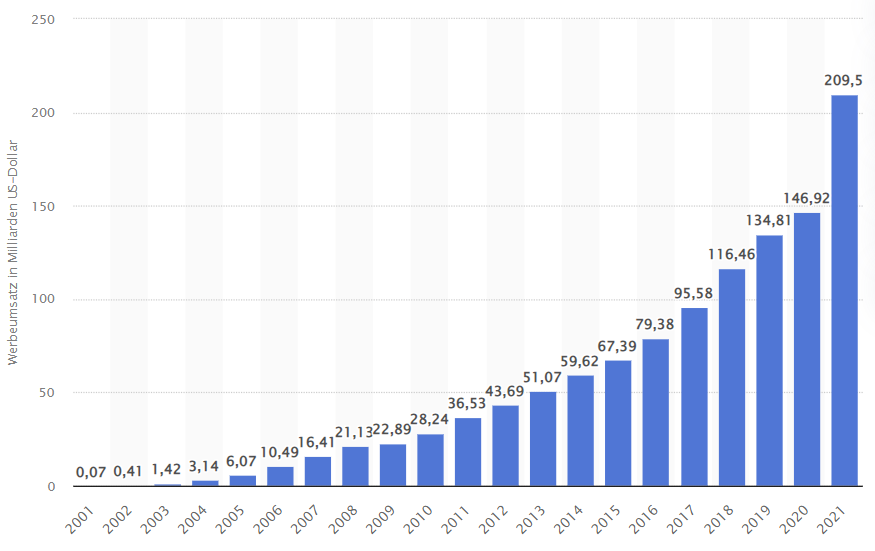
\includegraphics[width=120mm]{images/statistic_google_ads}
    \caption{Statistik Werbeumsätze Google in Milliarden}
    \label{fig:statisticAdsGoogle}
\end{figure}
Besonders in den letzten Jahren wurde auch personalisierte Werbung immer populärer.
Der Journalist und Author Dr. Björn Brückerhoff berichtet in einem Artikel 2020, wie Google Daten aus nahezu allen Anwendungen, sowie der Suchmaschine selbst und Betriebssystemen, wie in etwa Android, nutzt um Persönlichkeitsprofile seiner Nutzer zu erstellen.
Google kann laut Brückerhoff mit Hilfe dieser gigantischen Mengen an Daten auf \("\)Wünsche und Bedürfnisse,
die sexuelle Orientierung, die physische und psychische Gesundheit, die politischen Meinungen, die fnanziellen Möglichkeiten, die religiösen Überzeugungen oder die räumliche Flexibilität\("\)\cite{BRK20} schließen.
Mit Hilfe dieser Persönlichkeitsdaten platziert Google dann die mit Hilfe von Algorithmen ermittelte,
am besten auf uns zugeschnittene Werbung.\cite{BRK20}\\

Das Suchmaschinen-StartUp \("\)Qwant\("\) aus Frankreich gibt hingegen auf der Homepage der eigenen Suchmaschine nicht nur an,
keinerlei persönliche Daten zu verkaufen oder zu Werbezwecken zu nutzen, sondern auch diese persönlichen Daten nicht einmal zu erheben.
Die Suchmaschine finanziert sich laut Webseite \("\)kontextbasierte Werbung[, die] für alle gleich [ist]\("\)\cite{QWA22},
jeder sieht also, unabhängig vorherigen Suchen, die gleiche Werbung.

Bei Ergebnissen zu Suchanfragen kann bei den meisten Suchmaschinen, so auch bei Google,
Bing und Qwant zwischen \("\)Anzeigen\("\) und \("\)organischen Treffern\("\) unterschieden werden.
Anzeigen, auch unter dem Begriff \("\)Paid Listings\("\) bekannt, bezeichnen bezahlte Suchtreffer,
die von Suchmaschinen in die Suchergebnisse \("\)gemischt\("\) werden.
Solche Anzeigen müssen nach EU-Recht als solche gekennzeichnet werden.\\
Organische Treffer sind hingegen Treffer, die durch Algorithmen der Suchmaschine als am besten passend auf die aktuelle Suche bewertet werden.
In der folgenden Statistik wird die Anzahl der als \("\)Anzeige\("\) gekennzeichneten Treffern unter den ersten zehn Treffern auf ausgewählten Suchanfragen gezeigt.\cite{LEW18}\\
\begin{figure}[h]
    \centering
    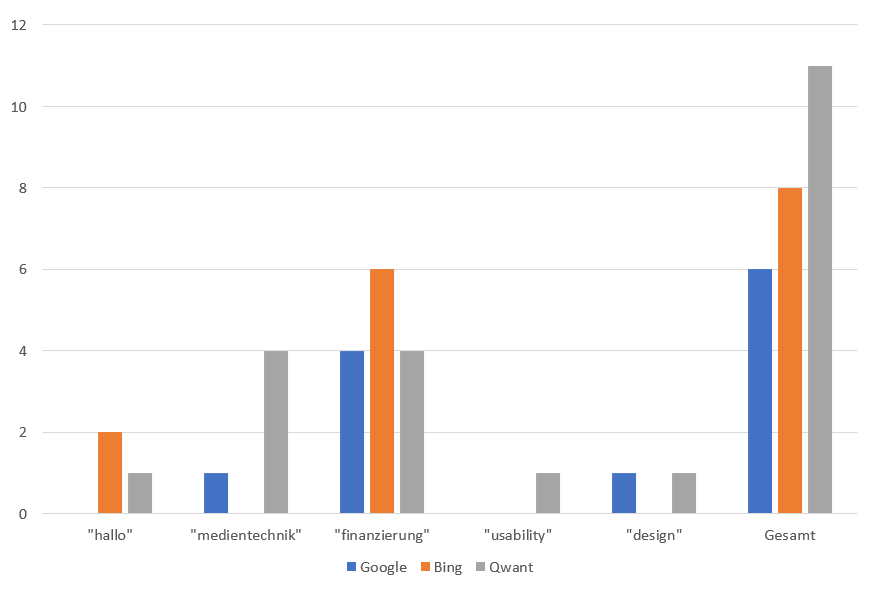
\includegraphics[width=120mm]{images/statistic_adverts}
    \caption{Statistik Anzeigen unter den ersten zehn Treffern bei ausgewählten Suchanfragen}
    \label{fig:statisticAdverts}
\end{figure}
Auffallend ist, dass Qwant insgesamt die meisten Anzeigen platziert hat, was allerdings daraus resultieren könnte,
dass es angibt keine Cookies wie Google und Bing zu verwenden, weshalb eine signifikante Einnahmequelle der Konkurrenz bei Qwant ausfällt.
Schaut man sich die Platzierungen der Anzeigen an, so fällt auf, dass Qwant diese oft,
im Gegensatz zu Bing und Google am Ende der aufgezeigten Suchergebnisse zeigt.
Auch fällt auf, dass der Anbieter mit den meisten Anzeigen bei fast jeder Anzeige sehr unterschiedlich ausfällt,
weshalb das Ergebnis auch stark von den gewählten Suchbegriffen abhängen könnte.\\
    \chapter{Usability}\label{ch:usability}

In diesem Kapitel wird die Usability anhand eines Usability Tests getestet.
Bei den Tests wird sich zur Vereinfachung der Vergleichbarkeit aud die Seiten google.de, bing.de, qwant.de beschränkt.
Auch wird sich bei der Einhaltung von Regeln und Gesetzen auf das deutsche Recht beschränkt.

\section{Test-Szenarien}\label{sec:szenarien}
Zur Durchführung wurden eine kleine Gruppe Informatik Studenten der \textbf{DHBW} gewählt.
Aufgrund mangelnder Ressourcen wurden diese in Eigenregie und ohne erstrebenswerte Tracking-Technologien wie z.B.\ Eye-tracking oder ähnliches durchgeführt.
Die Tester haben die Szenarien mit den drei verschiedenen Suchmaschinen \url{google.de} \url{bing.de} \url{qwant.de} durchgeführt,
und die Ergebnisse nach vorgegebenem Schema auf einer Skala von 1 bis 10 bewertet.

\subsection{Tag des Internets}\label{subsec:szenario1}
In diesem Szenario bekamen die Tester den Auftrag herauszufinden, wann der Tag des Internets ist.

\begin{tabular}{|c|c|c|c|}
    \hline
    & Dauer & Ergebnis & Selbsteinschätzung \\
    \hline
    Google & 10    & 10       & 10                 \\
    \hline
    Bing   & 9     & 9        & 8                  \\
    \hline
    Qwant  & 9     & 4        & 7                  \\
    \hline
\end{tabular}

\subsubsection*{Auswertung}
\paragraph{\url{google.de}}
hat durch die in der Mitte liegende Suchbar und das minimalistische Design,
sowie der sowieso sehr hohen Popularität eine schnelle Bedienbarkeit besonders bei einfachen Suchanfragen.\\

\paragraph{\url{bing.de}} hat durch die nicht ganz zentrale Suchleiste und das Design mit farbigem Hintergrundbild etwas länger gebraucht bis die Tester sich orientieren konnten.
Die Ergebnisseite von \url{google.de} und \url{bing.de} sind sich sehr ähnlich, siehe\nameref{fig:tag_des_internets_results}, weshalb dort auch von den Testern keine nennenswerten Unterschiede festzustellen waren.\\
\begin{figure}
    \centering
    \begin{minipage}[t]{0.45\linewidth}
        \centering
        \fbox{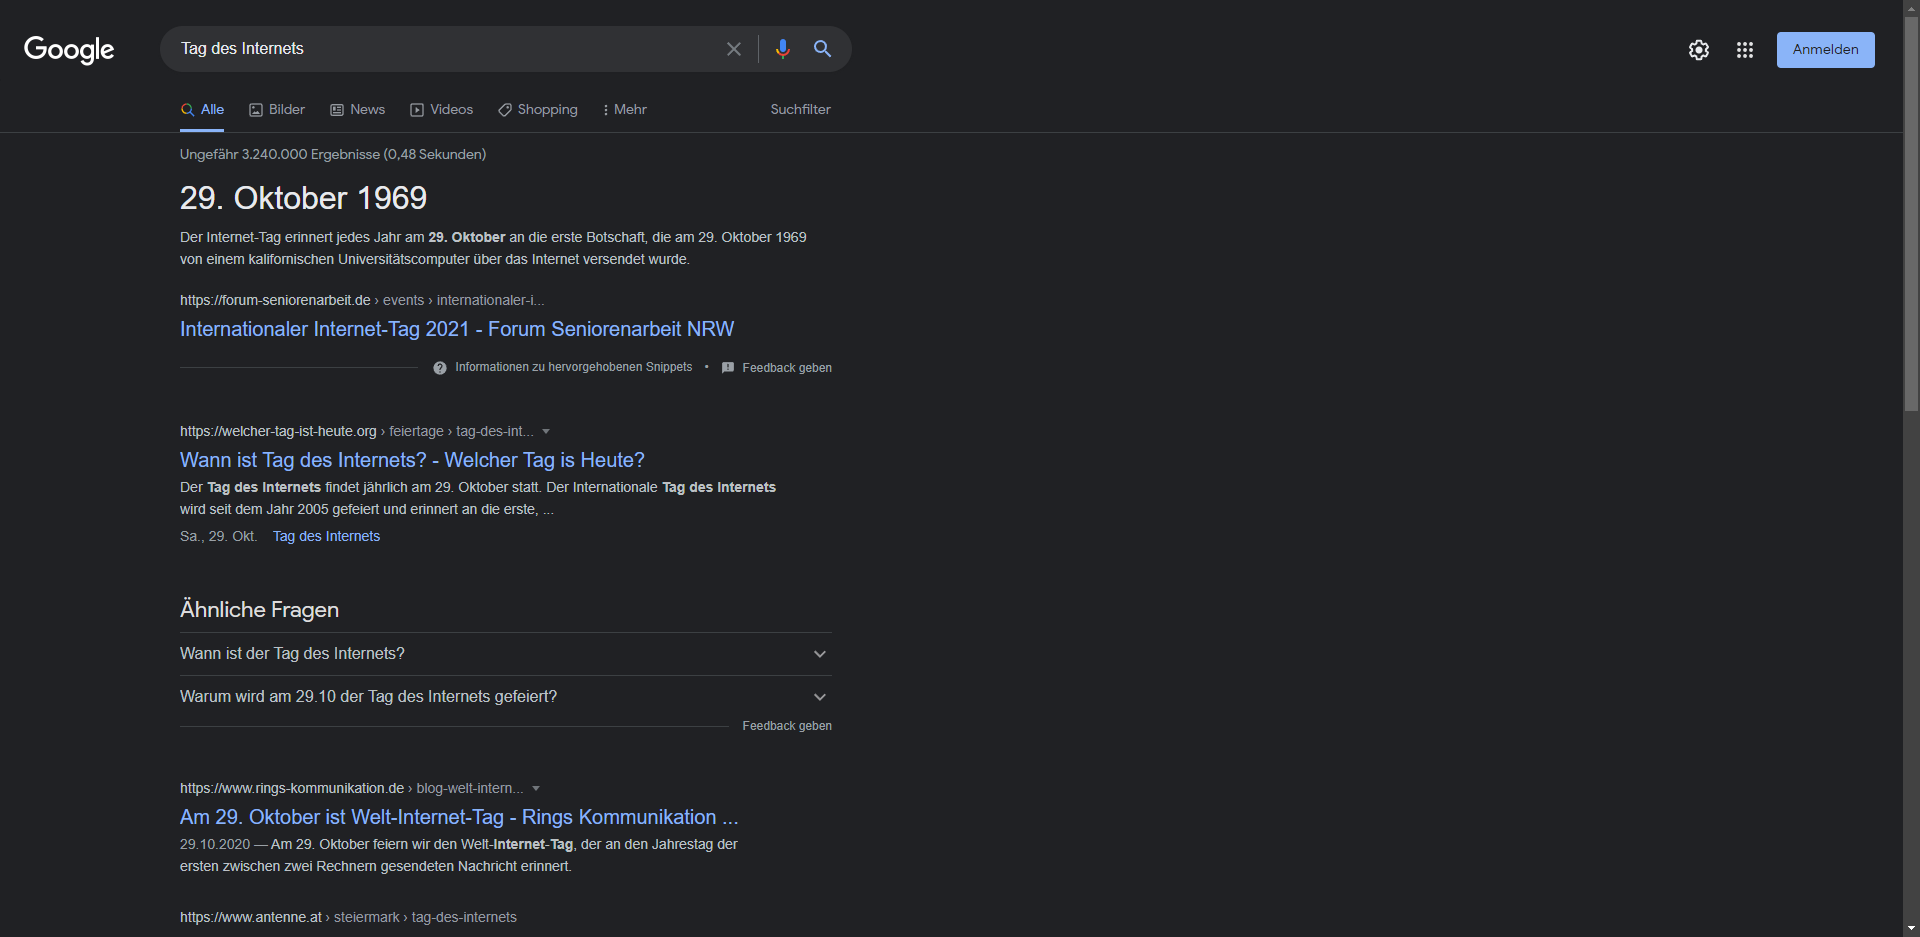
\includegraphics[width=\linewidth]{google_tag_des_internets_results}}
        Ergebnisse von \url{google.de}
    \end{minipage}%
    \hfill\vrule\hfill
    \begin{minipage}[t]{0.45\linewidth}
        \centering
        \fbox{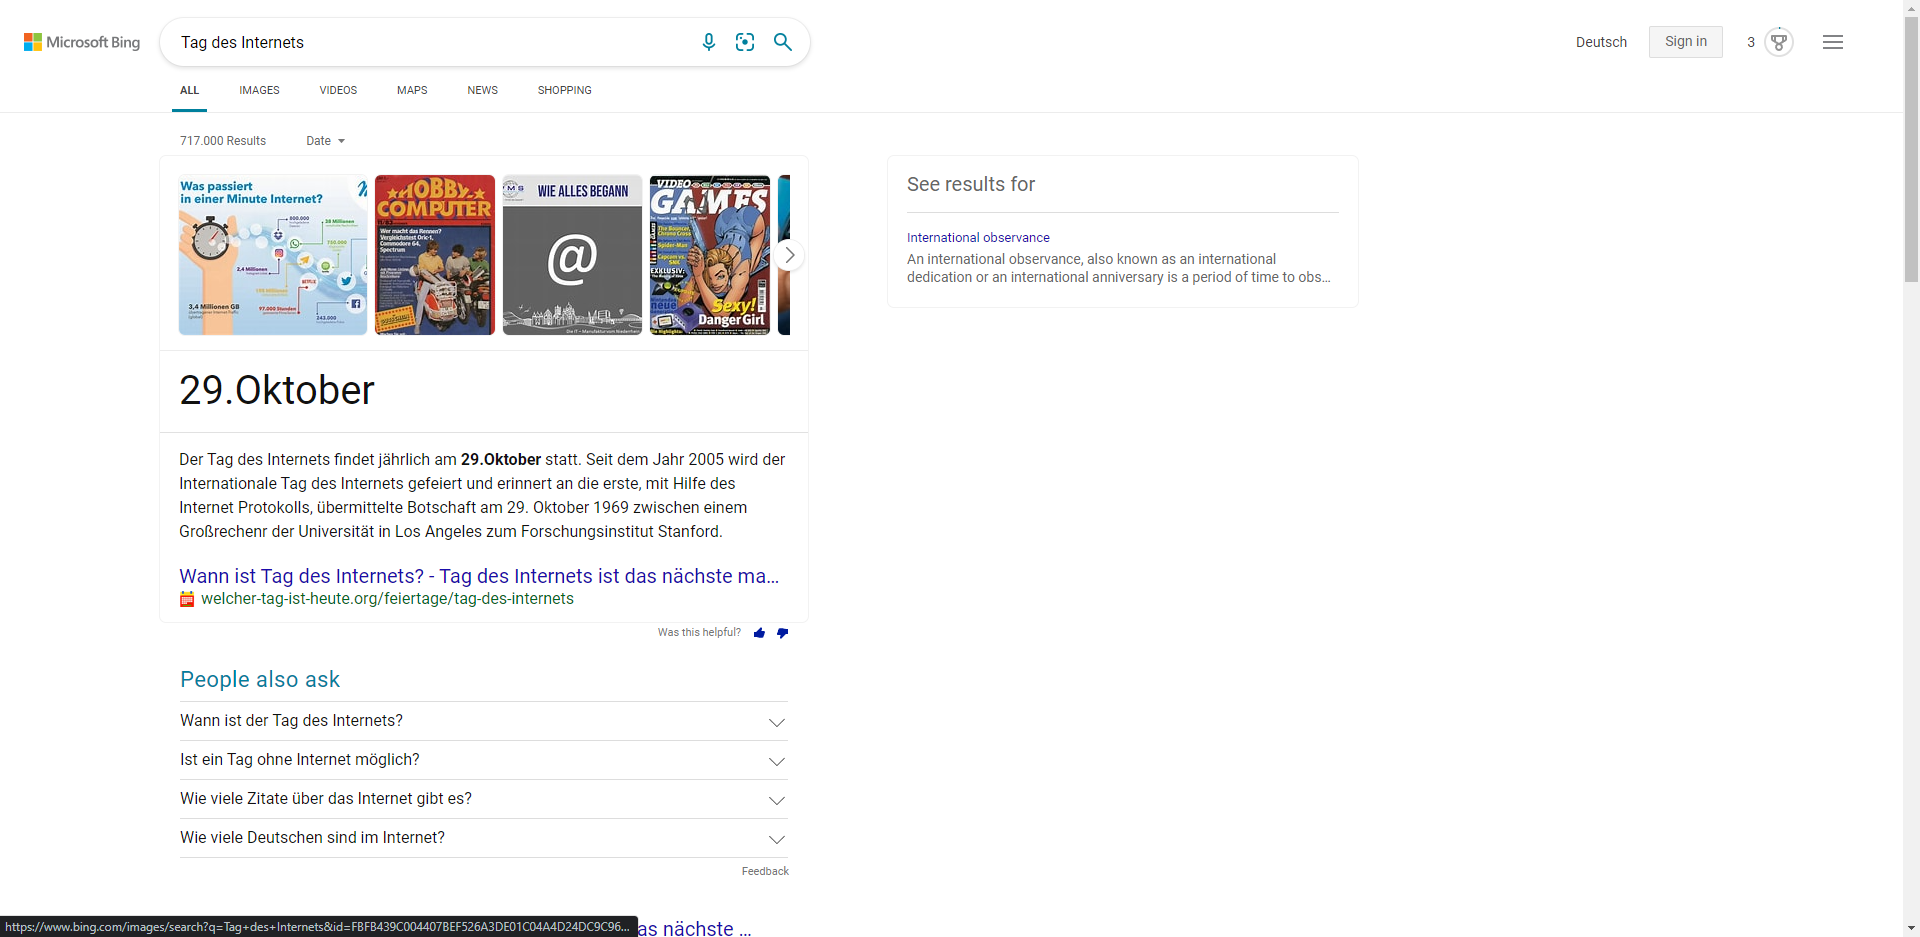
\includegraphics[width=\linewidth]{bing_tag_des_internets_results}}
        Ergebnisse von \url{bing.de}
    \end{minipage}
    \caption{Vergleich Ergebnis Google und Bing}\label{fig:tag_des_internets_results}
\end{figure}

\paragraph{\url{qwant.de}} hat bei den Testern eine lange Zeit gebraucht, um sich zu orientieren,
da das Design mit grellen Farben den Blick in die Mitte des Bildschirms gelockt hat und auch mehrere Knöpfe und Auswahlmöglichkeiten existieren.
Die hat es laut Aussagen der Tester erschwert, die Suchleiste in etwas dunklerem Design am oberen Bildschirmrand zu finden.
Auch die~\nameref{fig:qwant_tag_des_internets_results} ist nicht so gut wie bei \url{google.de} oder \url{bing.de},
da eine Übersicht mit dem Datum nicht direkt auf der Seite zu finden ist,
sondern erst in den Ergebnisseiten zu finden ist
\begin{figure}
    \centering
    \fbox{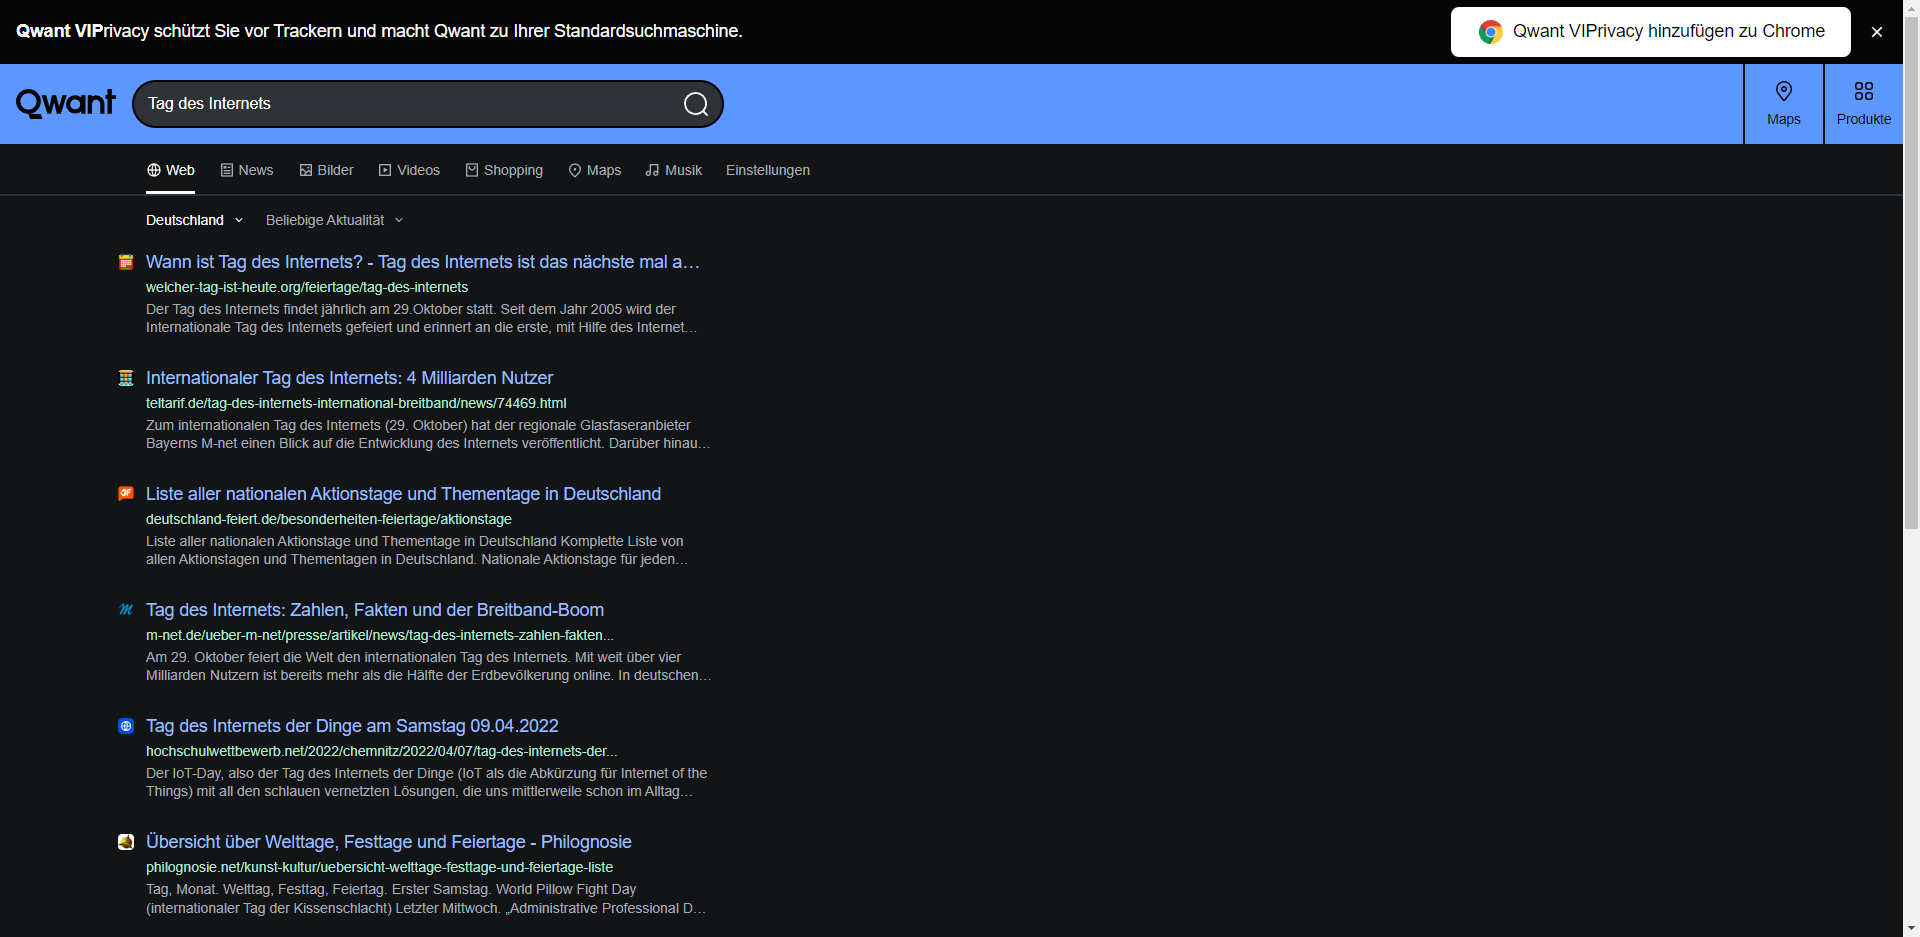
\includegraphics[width=0.5\linewidth]{qwant_tag_des_internets_results}}
    \caption{Ergebnisseite von \url{qwant.de}}\label{fig:qwant_tag_des_internets_results}
\end{figure}

\subsection{Katzenbild}\label{subsec:szenario2}
In diesem Szenario bekamen die Tester den Auftrag ein Katzenbild zu finden.

\begin{tabular}{|c|c|c|c|}
    \hline
    & Dauer & Ergebnis & Selbsteinschätzung \\
    \hline
    Google & 9     & 6        & 9                  \\
    \hline
    Bing   & 9     & 9        & 9                  \\
    \hline
    Qwant  & 10    & 8       & 10                 \\
    \hline
\end{tabular}

\subsubsection*{Auswertung}
\paragraph{\url{google.de}} zeigte den meisten Testern zwar direkt Katzenbilder an, jedoch nur wenige.
Die direkten Vorschaubilder waren meistens medizinische Katzenbilder und es gab neben dem kleinen Button Bilder, in der oberen Menüleiste, keine Möglichkeit mehr Bilder anzuzeigen.
Auch wenn dieser Button geklickt wurde gab es Probleme, da die erste Reihe Ergebnisse Werbung waren und auf diverse Online-Shopping Seiten weitergeleitet haben.\\

\paragraph{\url{bing.de}} hat dies deutlich besser gemacht und direkt als zweites Ergebnis den TEstern Bilder von Katzen geliefert.
Wenn die Tester diese angeklickt haben wurden sie auf die Bildergebnisseite weitergeleitet und das angeklickte Bild wurde groß und zentral angezeigt,
was es den Testern ermöglichte in kürzerer Zeit bessere Ergebnisse zu erzielen.\\

\paragraph{\url{qwant.de}} hat einen ähnlich guten Ansatz wie \url{bing.de} gewählt und präsentierte die Bilder direkt auf der Ergebnisseite sogar etwas weiter oben.

\subsection{Songtext}\label{subsec:szenario3}
In diesem Szenario bekamen die Tester den Auftrag den Songtext des Lieds Never gonna give you up von Rick Astley zu finden.

\begin{tabular}{|c|c|c|c|}
    \hline
    & Dauer & Ergebnis & Selbsteinschätzung \\
    \hline
    Google & 8     & 8       & 7                  \\
    \hline
    Bing   & 6     & 5        & 6                  \\
    \hline
    Qwant  & 6     & 5        & 6                  \\
    \hline
\end{tabular}

\subsubsection*{Auswertung}
%TODO Auswertung
\paragraph{\url{google.de}} hat die gemischtesten Ergebnisse geliefert.
Je nach Tester und Suchtext zeigte \url{google.de} entweder mehrere Ergebnisse an mit Webseiten,
auf denen die Liedtexte zu finden waren oder im besten Fall den kompletten Liedtext als erstes Ergebnis eingebettet.
\paragraph{\url{bing.de}} zeigte meist ein etwas hervorgehobenes Ergebnis als Erstes an, wo kleine Teile des Liedtextes zu sehen waren.
\paragraph{\url{qwant.de}} zeigte bei allen keine hervorgehobenen Ergebnisse an, sondern nur die gewöhnte Ergebnisseite.

\section{Accessibility}\label{sec:accessibility}
In diesem Kapitel wird die Accessibility getestet.
Es gibt einige Tests, die manuell und aufwändig getestet werden müssen.
Diese wurden nicht durchgeführt und es wurde sich auf die Ergebnisse der automatisierten Tests beschränkt.

Es werden die Guidelines der Web Accessibility Initiative (WAI) verwendet.
Diese Guidelines sind auf der Seite \url{https://www.w3.org/WAI/standards-guidelines/wcag/} verfügbar.\newline
Es wird unterschieden in folgende Level~\cite{WCAG21}:
\begin{itemize}
    \item Level A: niedrigstes Level der Accessibility.
    \item Level AA: mittleres Level der Accessibility.
    \item Level AAA: höchstes Level der Accessibility.
\end{itemize}

%TODO link to appendix

\subsection{Google}\label{subsec:google}
Wie in der Auswertung des Accessibility-Tests zu sehen ist, hat \url{google.de} mehrere Probleme mit der Accessibility.
Davon sind folgende Probleme als kritisch bewertet:
\begin{enumerate}
    \item Ein Button hat keinen besonderen Namen bekommen, wodurch es für Screenreader nicht möglich ist den Nutzern die Funktion des Buttons mitzuteilen.
    \item Der Kontrast zwischen Hintergrund und Vordergrund ist nicht ausreichend.
\end{enumerate}
Diese Probleme sind zwar als kritisch markiert, das Problem mit dem Button ist aber bei mehrfachen Tests nicht mehr aufgetreten.
Da minimale Kontraste in den WCAG 2.1-Guidelines erst für Level AA vorgeschrieben sind ist dies nicht fatal, sollte jedoch für ein Unternehmen wie Google durchaus erstrebenswert sein,
um die Benutzbarkeit für Menschen mit Sehbehinderung zu verbessern.

\subsection{Bing}\label{subsec:bing}
Wie in der Auswertung des Accessibility-Tests zu sehen ist, hat \url{bing.de} ein Problem mit der Accessibility.
Folgendes Problem wurde als kritisch bewertet:
\begin{enumerate}
    \item Die Zoomfunktion wurde in den meta-Tags deaktiviert.
\end{enumerate}
Dieses Problem scheint jedoch nur das Hintergrundbild zu betreffen, da das Interface vergrößert werden kann.
Aus diesem Grund ist das Problem als nicht kritisch zu betrachten, da die Benutzbarkeit für Menschen mit Sehbehinderung nicht beeinträchtigt wird.

\subsection{Qwant}\label{subsec:qwant}
Wie in der Auswertung des Accessibility-Tests zu sehen ist, hat \url{qwant.de} Probleme mit der Accessibility.
Folgende Probleme wurden als kritisch bewertet:
\begin{enumerate}
    \item Ein Button hat keinen besonderen Namen bekommen, wodurch es für Screenreader nicht möglich ist den Nutzern die Funktion des Buttons mitzuteilen.
    \item Der Linktext einiger Elemente ist nicht eindeutig.
\end{enumerate}
Das Problem mit den Nicht eindeutig benannten Elementen ist auch bei mehrfachen Tests aufgetreten.
Da eindeutige Namen in den WCAG 2.1-Guidelines für Level A vorgeschrieben sind siehe `Success Criterion 1.1.1 Non-text Content`\cite{WCAG21},
ist dies eine klare Verletzung der WCAG 2.1 A Guidelines, wodurch sich \url{qwant.de} nicht für eine Accessibility-Kompatibilität laut WCAG 2.1-Guidelines qualifiziert.

\section{Vergleich}\label{sec:vergleich}
In diesem Kapitel werden die Ergebnisse der selbst durchgeführten Tests,
sowie der automatisierten Accessibility-Tests zusammengeführt, abstrahiert und in Perspektive gesetzt.
In~\nameref{fig:google_home},~\nameref{fig:bing_home} und~\nameref{fig:qwant_home} sind die Startseiten der jeweiligen Seiten zu sehen.\\

Nach Abschluss der Accessibility Tests ist zu sagen,
dass aus Accessibility Sicht sich die etablierten Suchmaschinen \url{google.de} und \url{bing.de} nicht sehr unterscheiden.
Beide haben zwar Probleme mit der Benennung der Knöpfe und Bilder, was für Screenreader und Menschen mit Sehbehinderung nicht optimal ist.
Erfüllen jedoch den WCAG 2.1 A Standard.
Um die Accessibility zu verbessern, sollten die Seiten jedoch kontrastreicher gestaltet werden.\\

\url{qwant.de} hat jedoch klare Probleme mit der eindeutigen Benennung von Knöpfen und Linktexten, was an der Überladung der Seite liegt.
So sieht man zum Beispiel in~\nameref{fig:qwant_home}, dass der User neben den notwendigen Elementen,
wie einer Suchleiste, Einstellungen und eventuell weiteren Produkten des Unternehmens mit zu vielen Informationen überschüttet wird.
Um die Accessibility zu verbessern, sollte die Seite ihr Design vereinfachen und sich auf der Startseite auf die zur Funktionalität beitragenden Elemente beschränken.


\begin{figure}[h]
    \centering
    \fbox{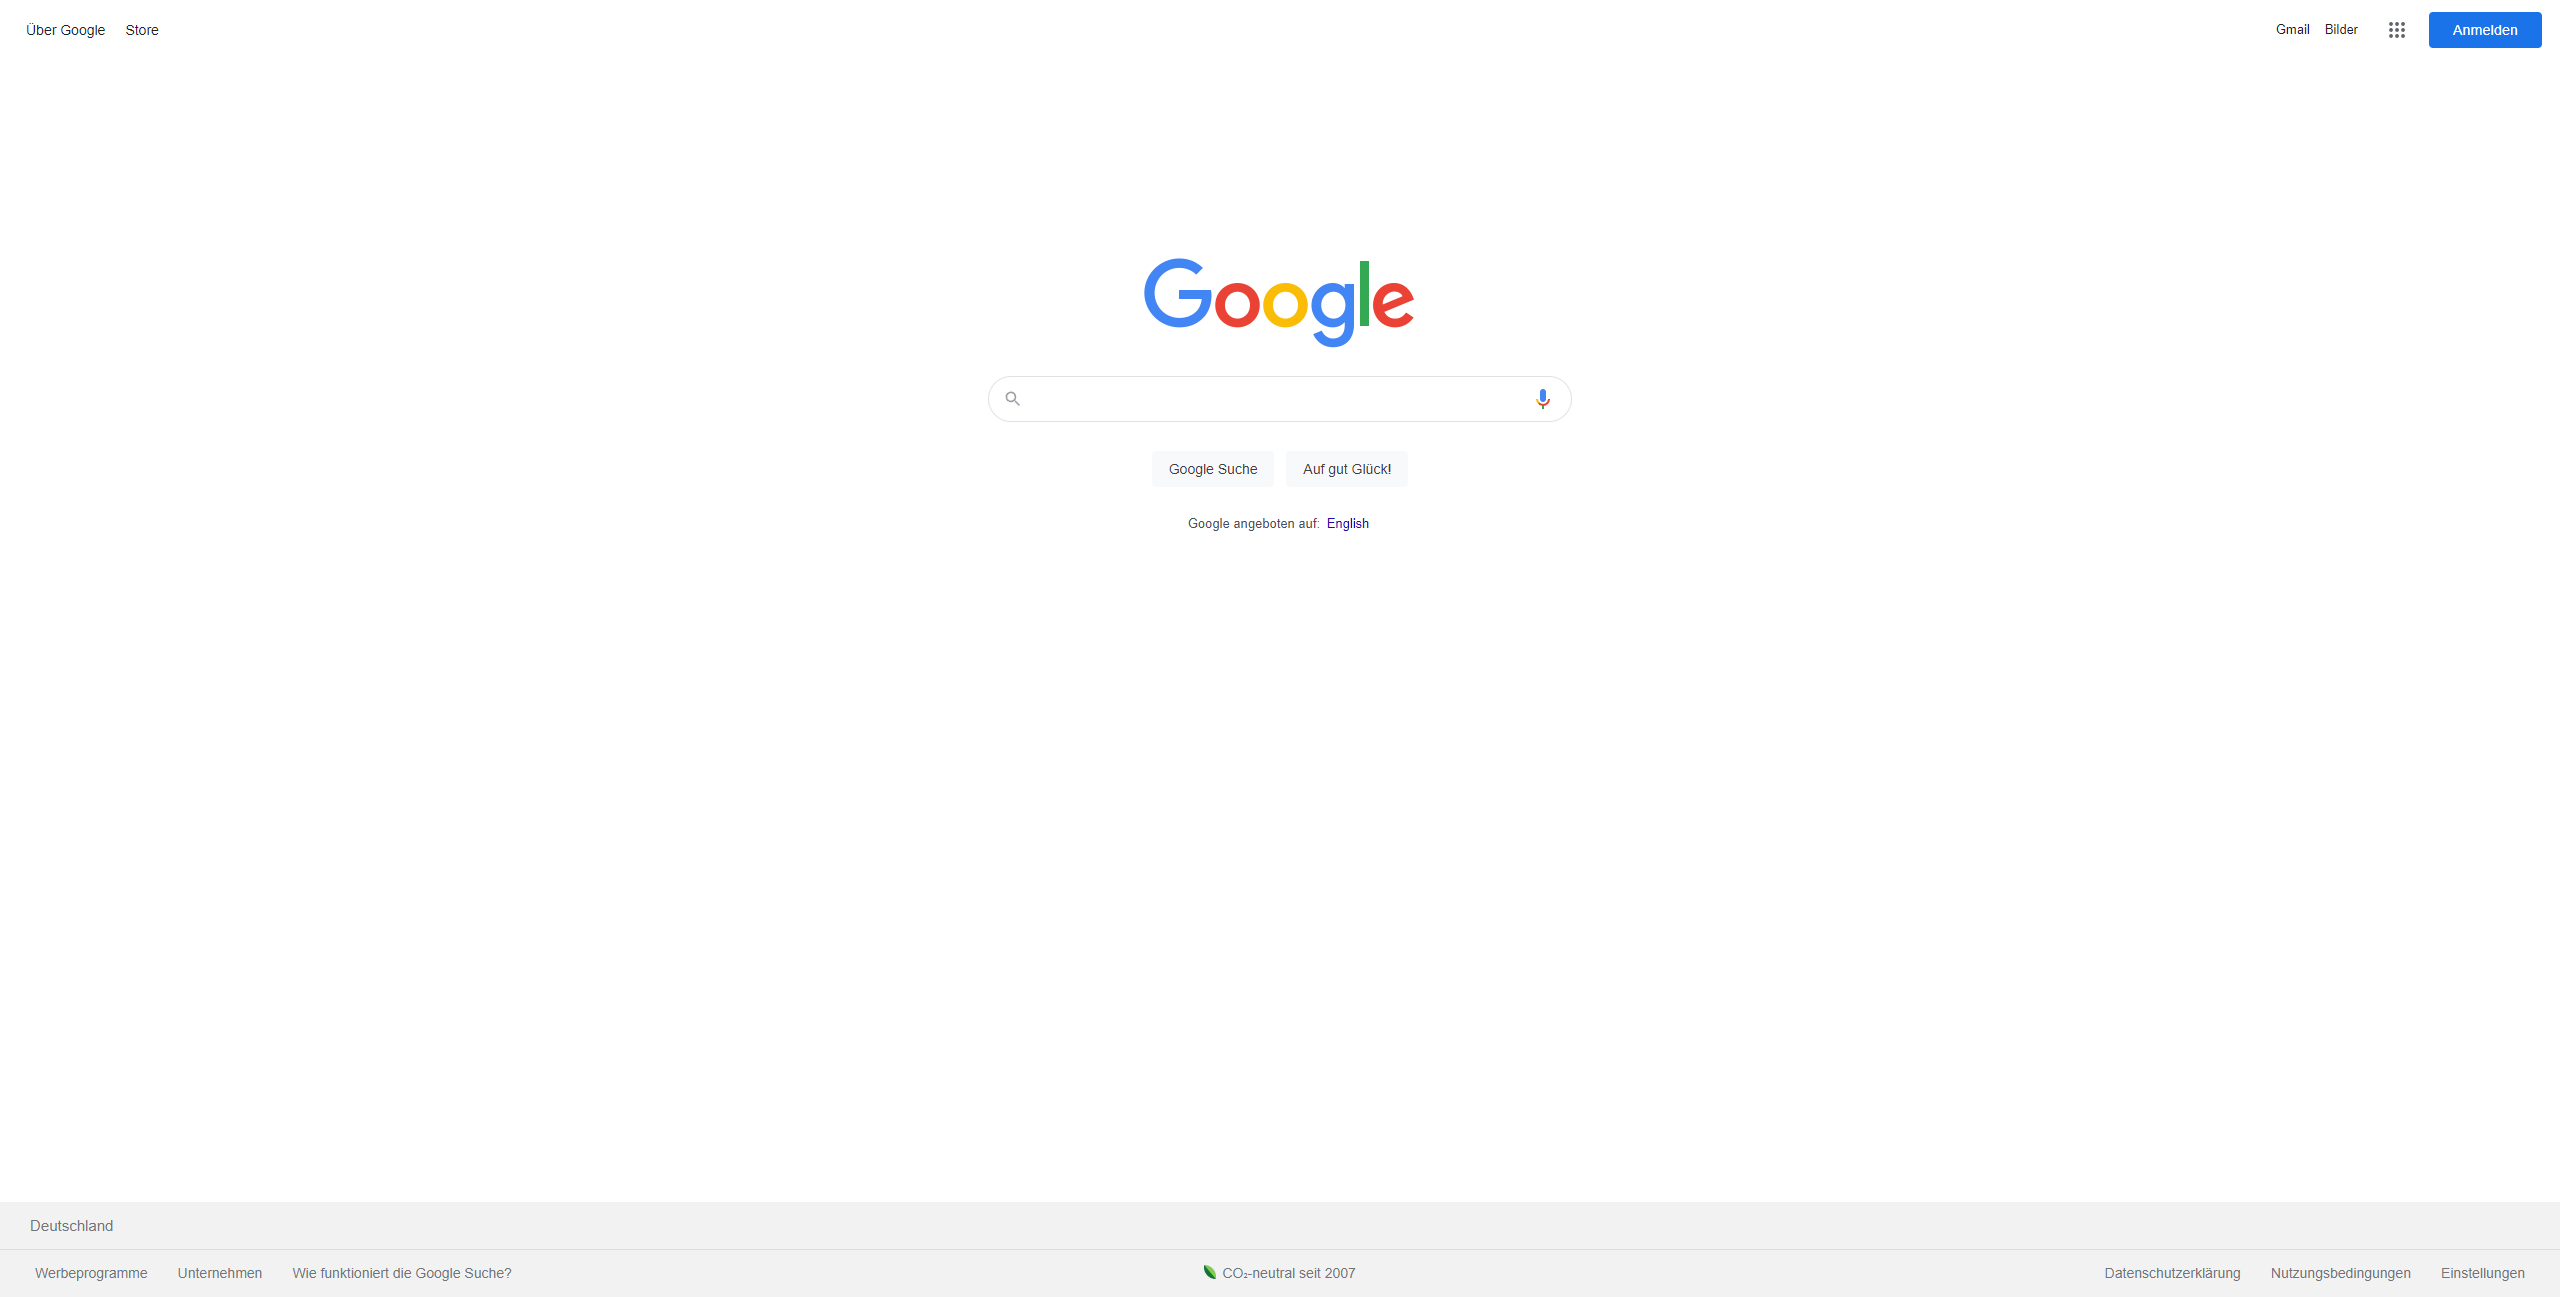
\includegraphics[height=0.3\textheight]{google_home}}\caption{Google Home}\label{fig:google_home}
\end{figure}
\begin{figure}[h]
    \centering
    \fbox{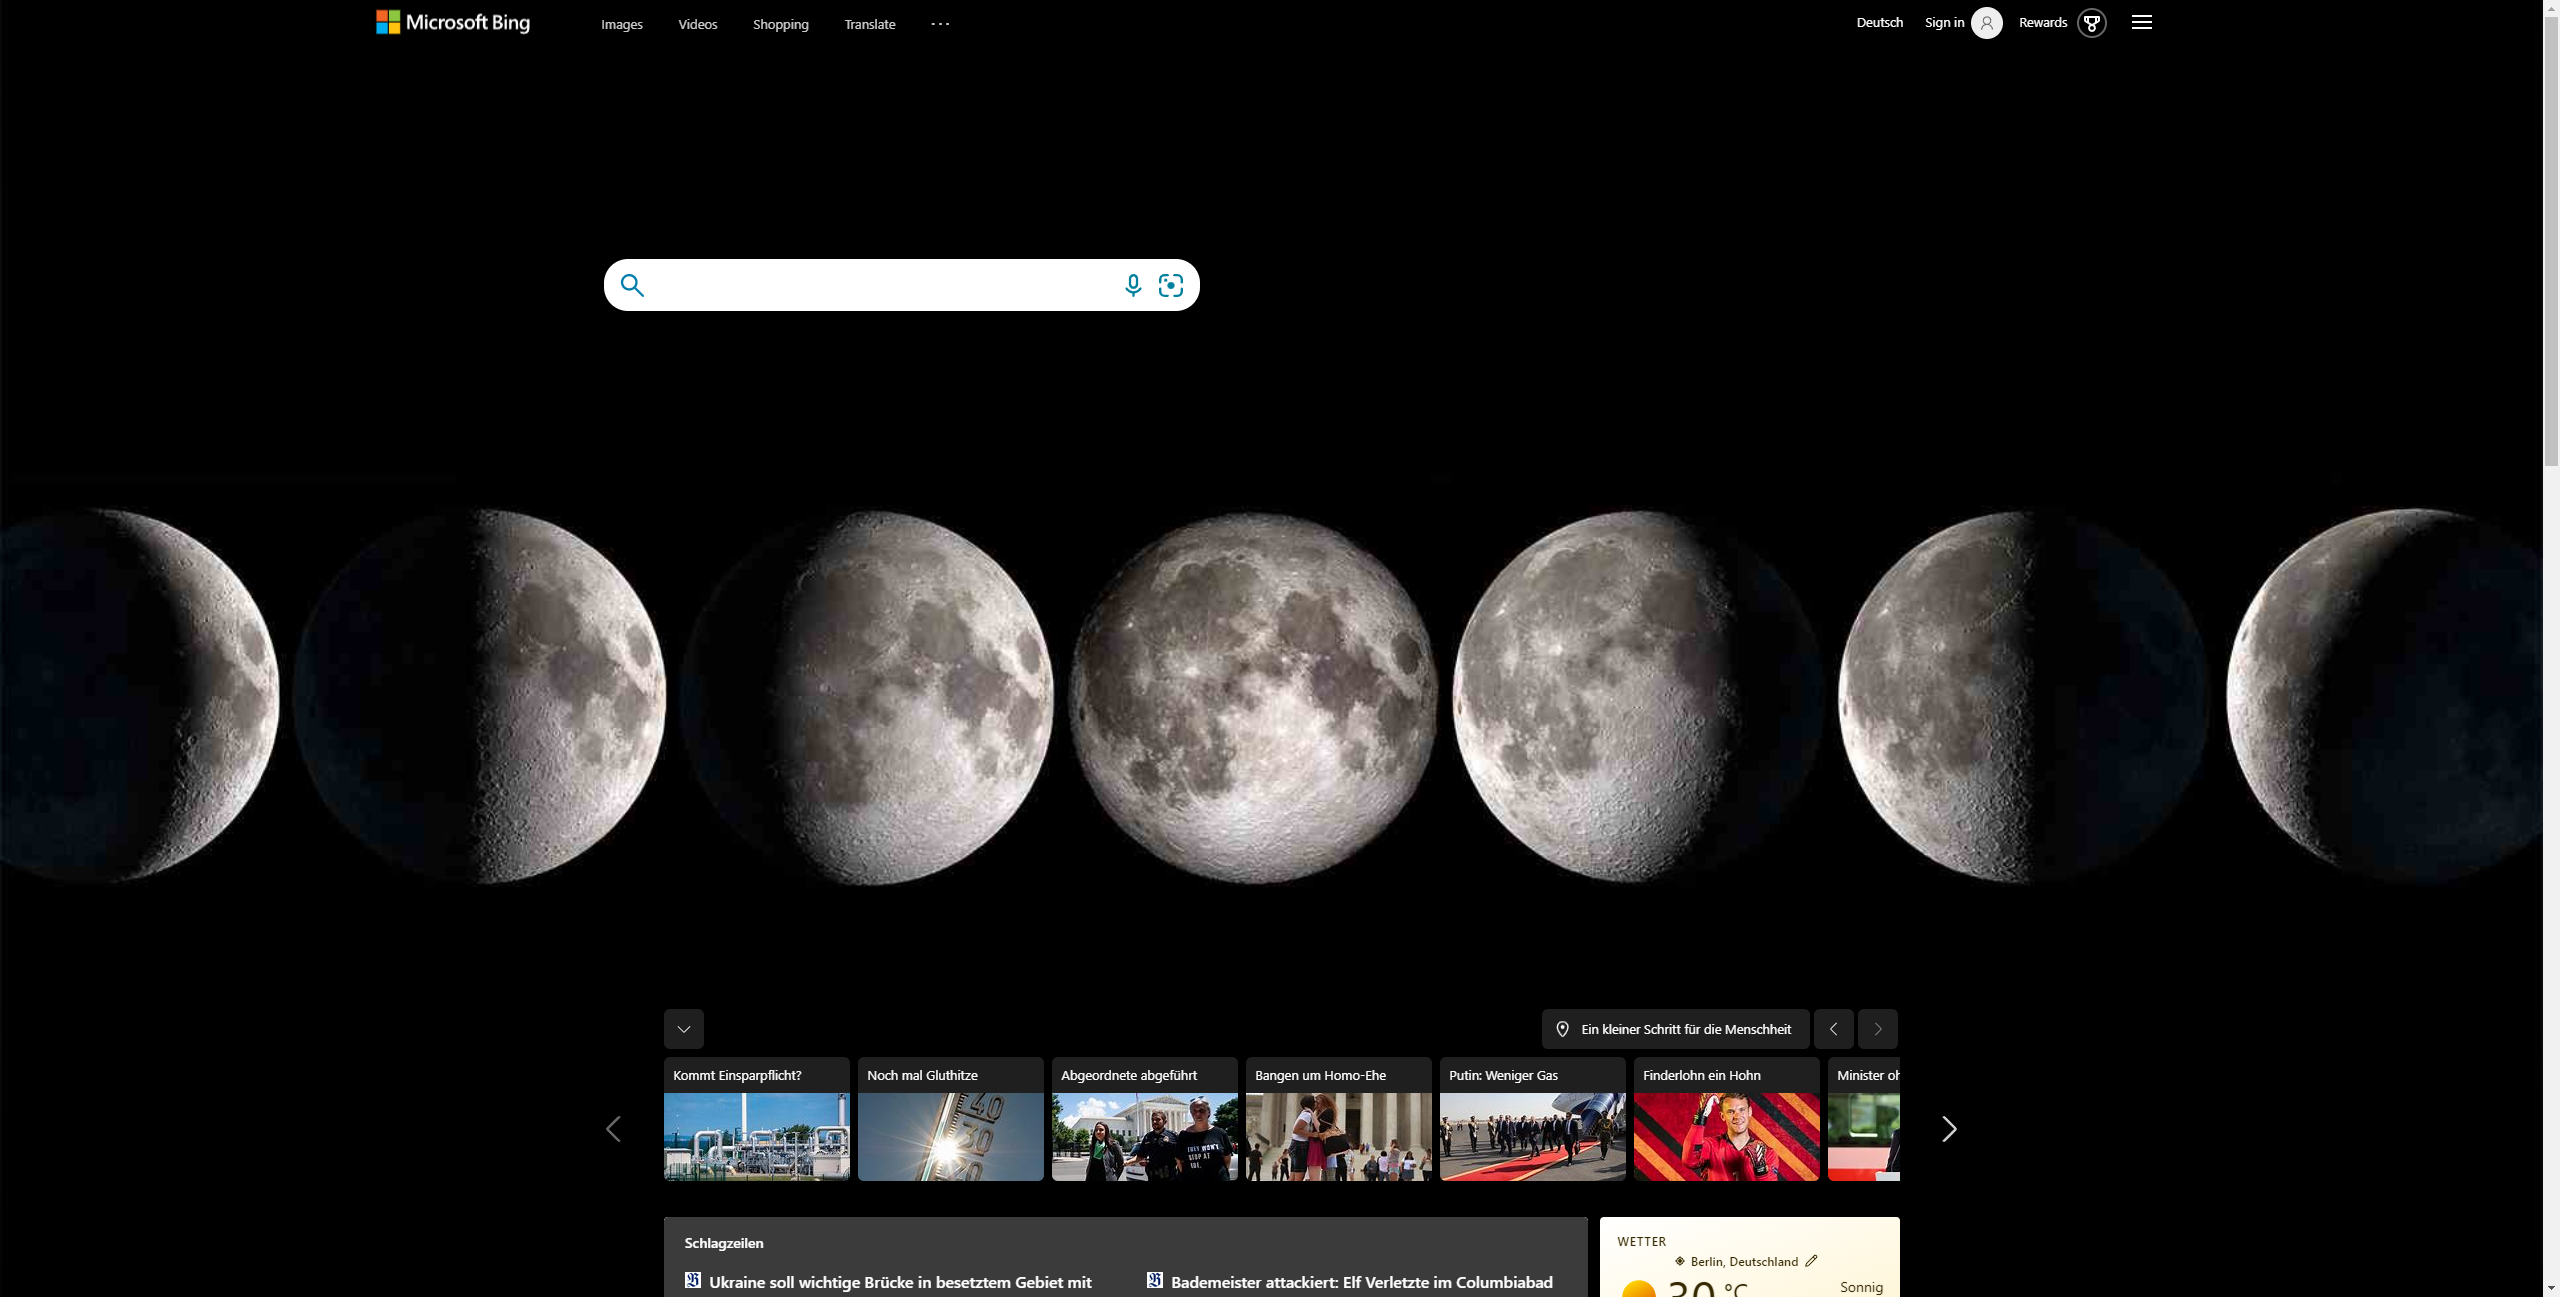
\includegraphics[height=0.3\textheight]{bing_home}}\caption{Bing Home}\label{fig:bing_home}
\end{figure}
\begin{figure}[h]
    \centering
    \fbox{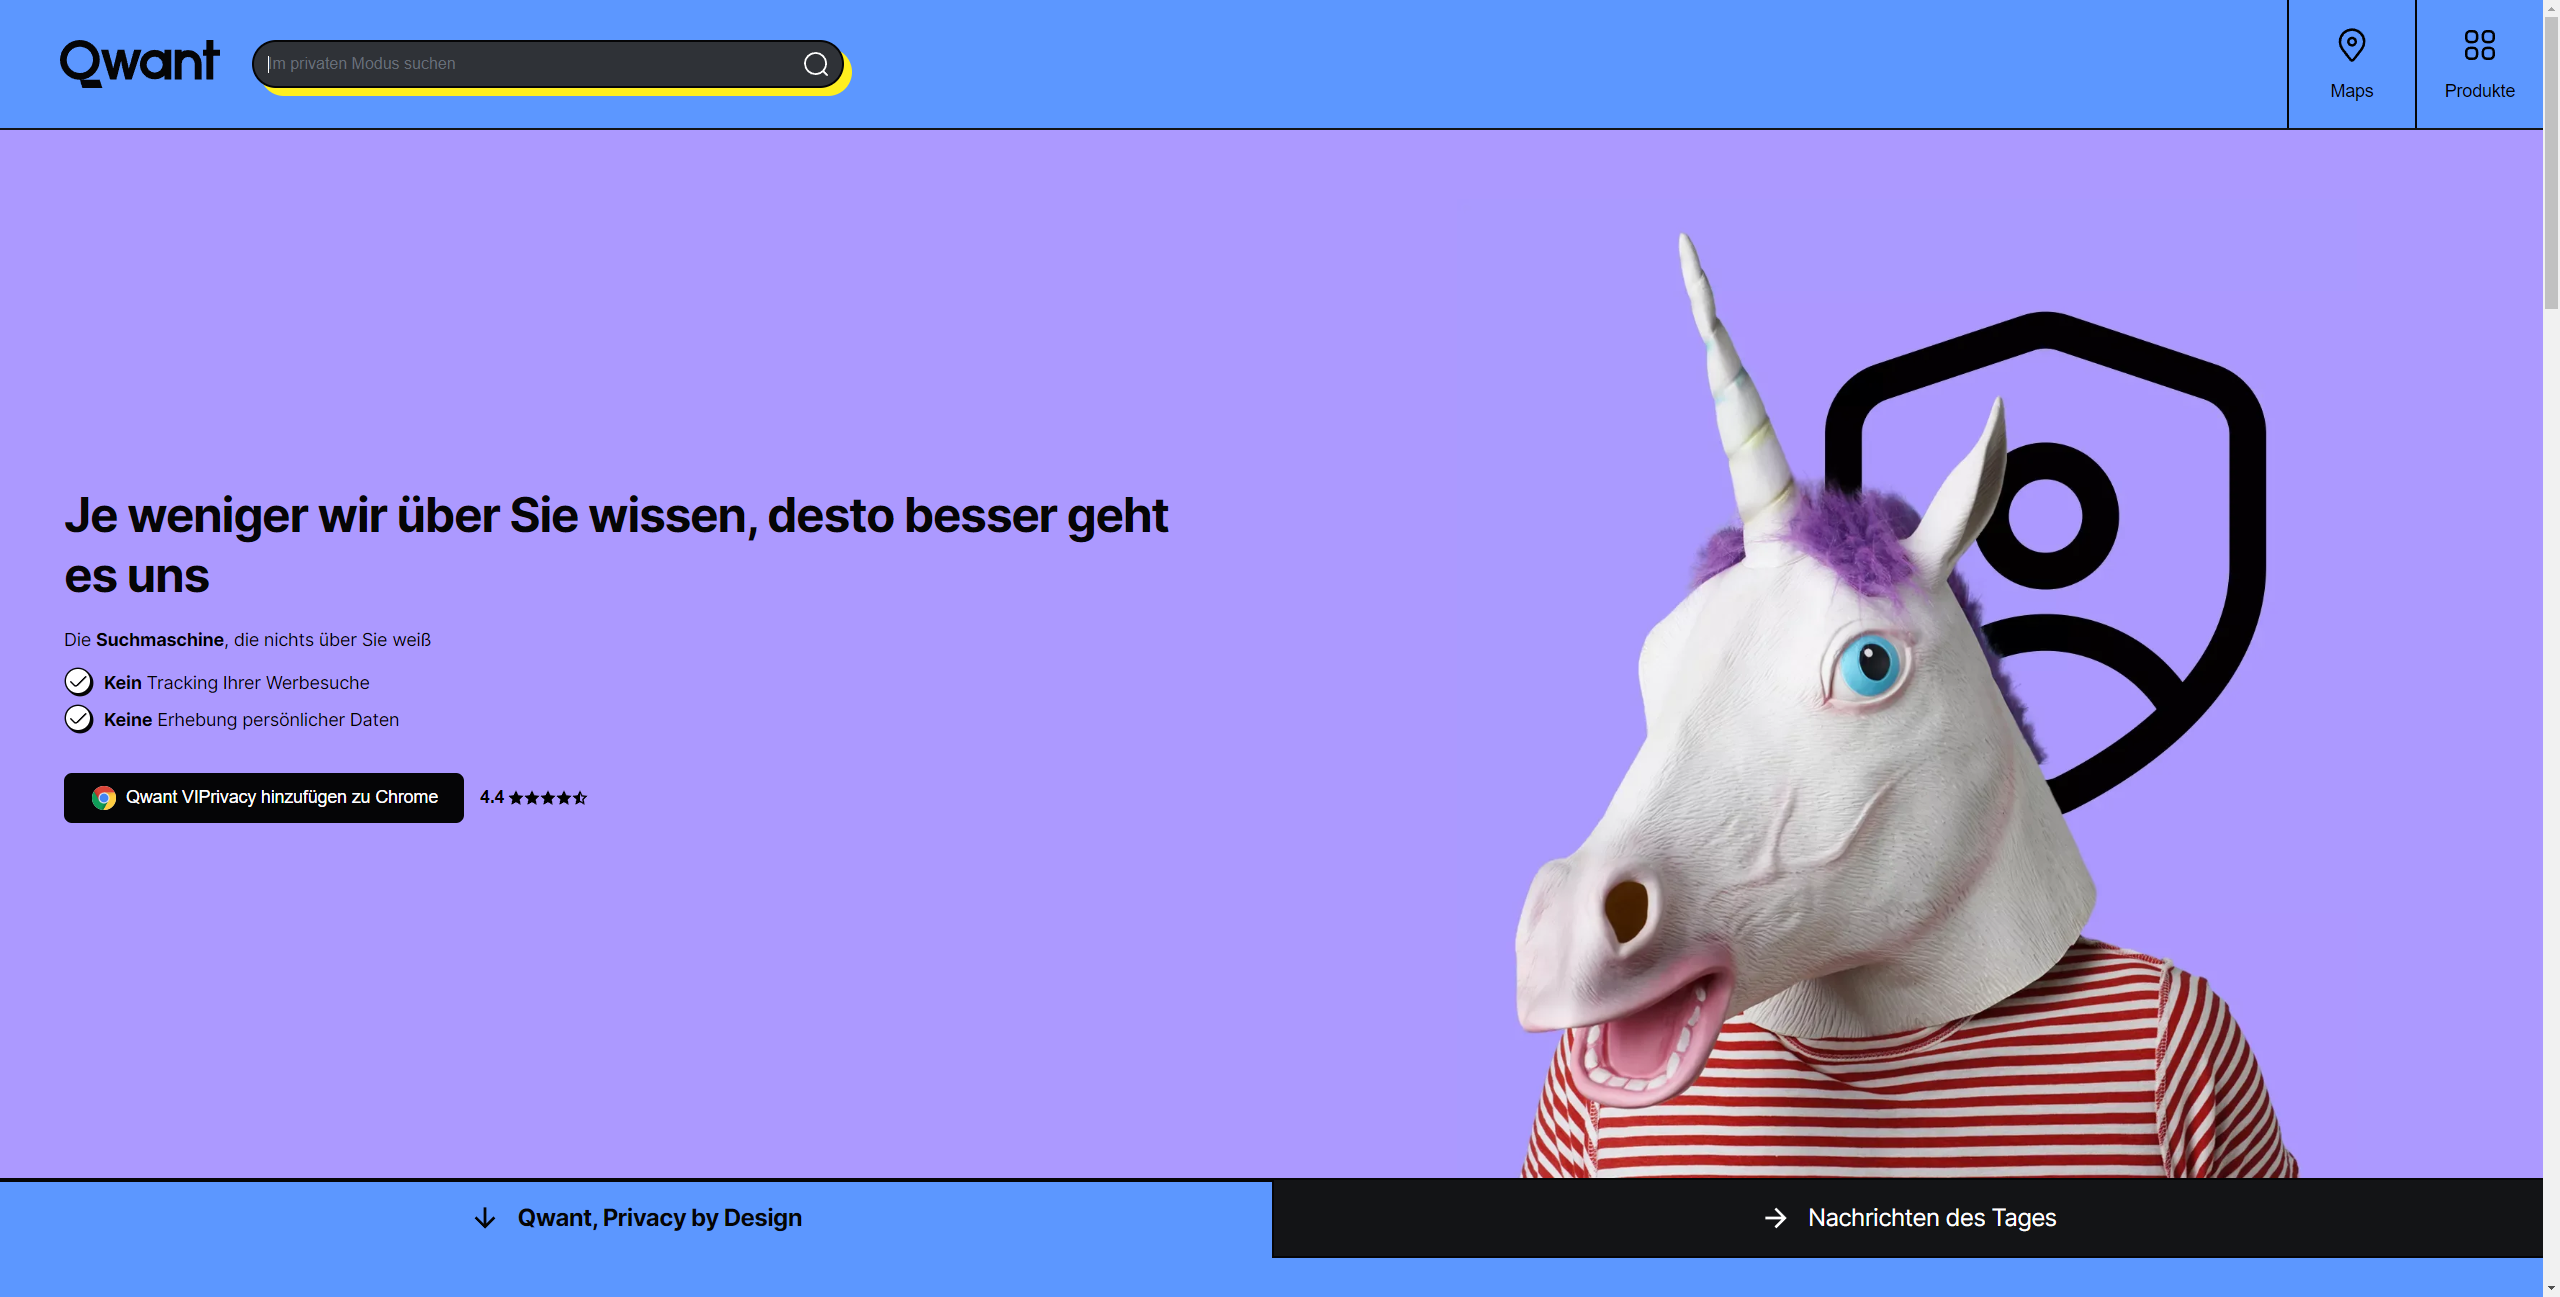
\includegraphics[height=0.3\textheight]{qwant_home}}\caption{Qwant Home}\label{fig:qwant_home}
\end{figure}
    \section{Wie uns Google beeinflusst}\label{sec:wie-uns-google-beeinflusst}

\subsection{Der Einfluss von Google}\label{subsec:der-einfluss-von-google}
Mit einem Marktanteil von über 90 Prozent in Deutschland, im mobilen Sektor sogar über 96 Prozent, erfreut sich die Google Suchmaschine in den letzten Jahren immer größerer Beliebtheit.
Während das Rennen der Suchmaschinen vor etwa 20 Jahren noch ein \("\)bunte Mischung\("\) war, hat Google heute nahezu ein Monopol in diesem Bereich geschaffen.
Auch weltweit ist Google, wenn auch nicht so eindeutig wie das in Deutschland der Fall ist, mit Abstand auf Platz eins der beliebtesten Suchmaschinen.
Jeder von uns \("\)googelt\("\)\cite{DUD22}, wie es die Suchmaschine schon in den deutschen Duden geschafft hat, im Schnitt dreimal am Tag.\cite{DOL22}\\
Wenn man diese Zahlen hört, dürfte schon klar sein, dass Google unser Verhalten als Nutzer im Web maßgeblich beeinflusst hat.
Wie genau Google uns beeinflusst hat oder vielleicht noch beeinflussen wird, wird im Folgenden analysiert.

\subsection{Veränderung des Benutzerverhaltens mehrerer Generationen}\label{subsec:veränderung-des-benutzerverhaltens-mehrerer-generationen}
Modernisierung des Webs - das Google-Ranking bestimmt, ob und auf welchem Platz eine Webseite dem Nutzer bei einer Suchanfrage vorgeschlagen wird.
Um in diesem Ranking möglichst gut platziert zu werden, sollte man bestimmte Voraussetzungen erfüllen, so sei es beispielsweise wichtig die Webseite gut an die Ansicht auf Mobilen Geräten anzupassen.\cite{BUI22}
Wie eine Statistik von statcounter zeigt, übertraf die Internetnutzung auf mobilen Geräten 2016 erstmals die Nutzung von einem Desktop aus mit einem ständigen Wachstum der mobilen Nutzung seit 2009.\cite{STA16}
Nicht zuletzt dürfte dazu wohl auch die immer besser werdende Benutzerfreundlichkeit von Webseiten auf mobilen Geräten beigetragen haben.
Und weil Seiten mit einer guten Anpassung auf mobile Geräte von Google höher gerankt werden, ist es wohl kein Wunder, dass wir unsere mobilen Geräte auch für das surfen im Netz immer mehr benutzen können.
Auch in Zukunft, wenn der Trend weiter in Richtung mobile Geräte, wie eventuell auch SmartWatches oder Sprachsteuerung geht,
wird Google wohl signifikant mitbestimmen, inwieweit das World Wide Web zugänglich für neue Technologien wird.\\

Informationsbeschaffung - Informationsquellen, die Quellen, aus denen wir unser Individualwissen nehmen,
veränderten und vermischten sich in der Geschichte immer wieder aufs Neue.
Von reiner mündlicher Überlieferung über Buchdruck und Radio bis zum Fernsehen.
Doch wohl kaum gab es zuvor eine Quelle mit der man so schnell Informationen in vergleichbaren Mengen und aus vergleichbar vielen Quellen beschaffen konnte wie mit dem Internet.
Einem Bericht der \("\)mednic\("\) zufolge gaben 82 Prozent der Befragten 2020 an sich über Covid-19 im Internet zu informieren.\cite{RKW20}
Ob über Nachrichtenseiten, Social Media oder Podcasts und egal über welches Thema,
Google und Co liefern uns Informationen und vor allem in jüngeren Generationen werden Suchmaschinen eine immer beliebtere Informationsquelle.\\

Konnektivität der Google Dienste - ob die Google Suchmaschine, Gmail, YouTube, Maps oder den Google Play Store,
die meisten von uns nutzen nicht nur eines der zahlreichen Google Produkte und Dienste.
In der Gmail-App kann man ganz einfach mithilfe von Google Drive auch größere Dateien anhängen und in der Google Suchmaschine kann man ganz einfach seinen YouTube und Gmail Account einbinden, alles mit Hilfe des Google Kontos.
Und das sind nur ein paar Beispiele, wie man verschiedenste Google Dienste vergleichsweise einfach miteinander verbinden kann.
\begin{figure}[ht]
    \centering
    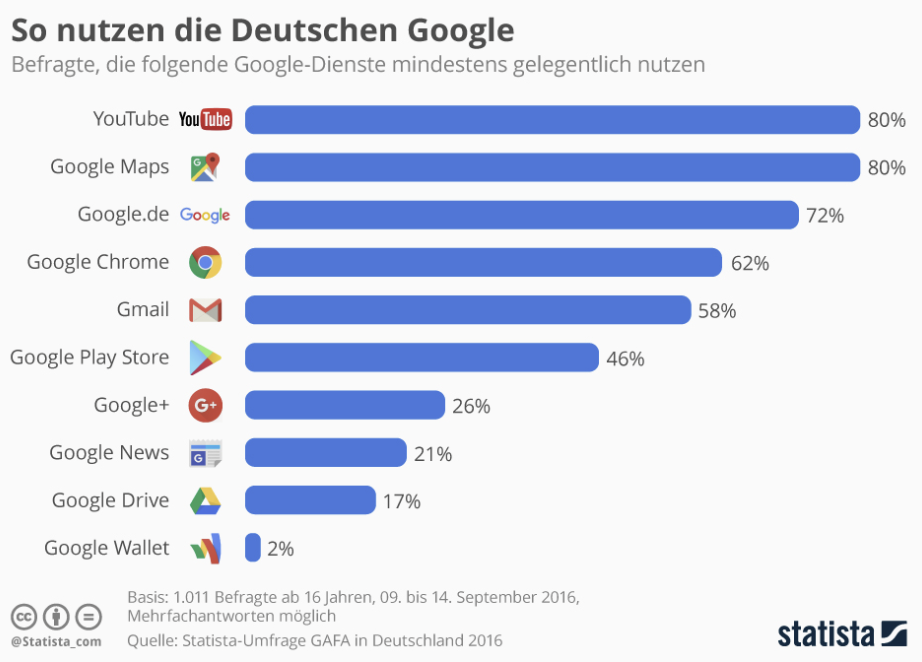
\includegraphics[width=100mm]{images/statistic_googleServices}
    \caption{Statistik Nutzung der Google Dienste in Deutschland}
    \label{fig:statisticGoogleServices}
\end{figure}  %https://de.statista.com/infografik/6020/nutzung-von-google-diensten-in-deutschland/
Wie in der Statistik zu sehen ist, nutzen bereits heute 80 Prozent der Menschen in Deutschland Google Maps und YouTube, dicht gefolgt von der Google Suchmaschine mit 72 Prozent.
Auch die restlichen Google Services sind in Deutschland gut vertreten und das wohl nicht zuletzt auch,
weil Google es uns in den letzten Jahren immer einfacher gemacht hat die verschiedenen Dienste miteinander zu verbinden.
Erst 2019 wurde Google+, was immerhin 26 Prozent der Deutschen nutzten, eingestellt.
Bei dem Google Dienst, der gerade einmal knapp 8 Jahre am Markt war, handelte es sich um ein soziales Netzwerk,
das \("\)mehrere Google-Werkzeuge [\ldots] in einem einzigen sozialen Netzwerk von Google\("\)\cite{JEC21} vereinen sollte.\cite{JEC21}
Und, auch wenn dieses Projekt gescheitert ist, sieht man daran, wie Google immer wieder versucht seine Dienste noch besser miteinander zu vernetzen.
Schon heute haben sich die Google features wie wohl kaum eines anderen Anbieter in unseren Alltag integriert,
und so wird Google wohl auch in Zukunft, wenn es vielleicht noch weitere Google Dienste geben wird, durch gute Konnektivität und eine dadurch verbesserte User Experience überzeugen.\\

UX und Einfachheit - Eine schlichte, meist weiße Webseite mit einer Suchbar in der Mitte und einem kleinen Bild darüber,
in den Grundzügen sieht die Landingpage der Google Suchmaschine schon seit es sie gibt so aus.
Mit kleinen der Zeit angepassten Modernisierungen selbstverständlich.
Die Nutzung der Google Suchmaschine könnte wohl kaum einfacher und selbsterklärender sein.
Usability beschreibt die Nutzbarkeit oder auch Gebrauchstauglichkeit eines Produktes und ist ein wesentlicher Bestandteil der UX (=User Experience),
die wiederum beschreibt wie gut die Erfahrung ist, die ein User mit dem Produkt im Durchschnitt macht, also wie einfach und komfortable ein Produkt für der User oder Anwender nutzbar ist.\cite{Maulhardt4}
Durch die einfache und selbsterklärende Nutzung weißt Google eine ziemlich hohe Usability vor und nicht nur das,
die Usability ist auch ein wesentlicher Bestandteil des Rankings von Google, so gibt uns Google bevorzugt Ergebnisse aus, bei denen die Usability auch vergleichsmäßig hoch ist,
was ein weiterer Grund ist warum viele die Suchergebnisse von Google sehr schätzen und wohl auch in Zukunft noch schätzen werden.\cite{LIC15}\\

Accessibility der Information - Das Ziel, das die Google Suchmaschine von Anfang an verfolgt hat,
ist es Informationen für Menschen erreichbar zu machen und die Benutzer sind es gewohnt und erwarten auch schnell und einfach an die Information zu kommen.
\begin{figure}[h]
    \centering
    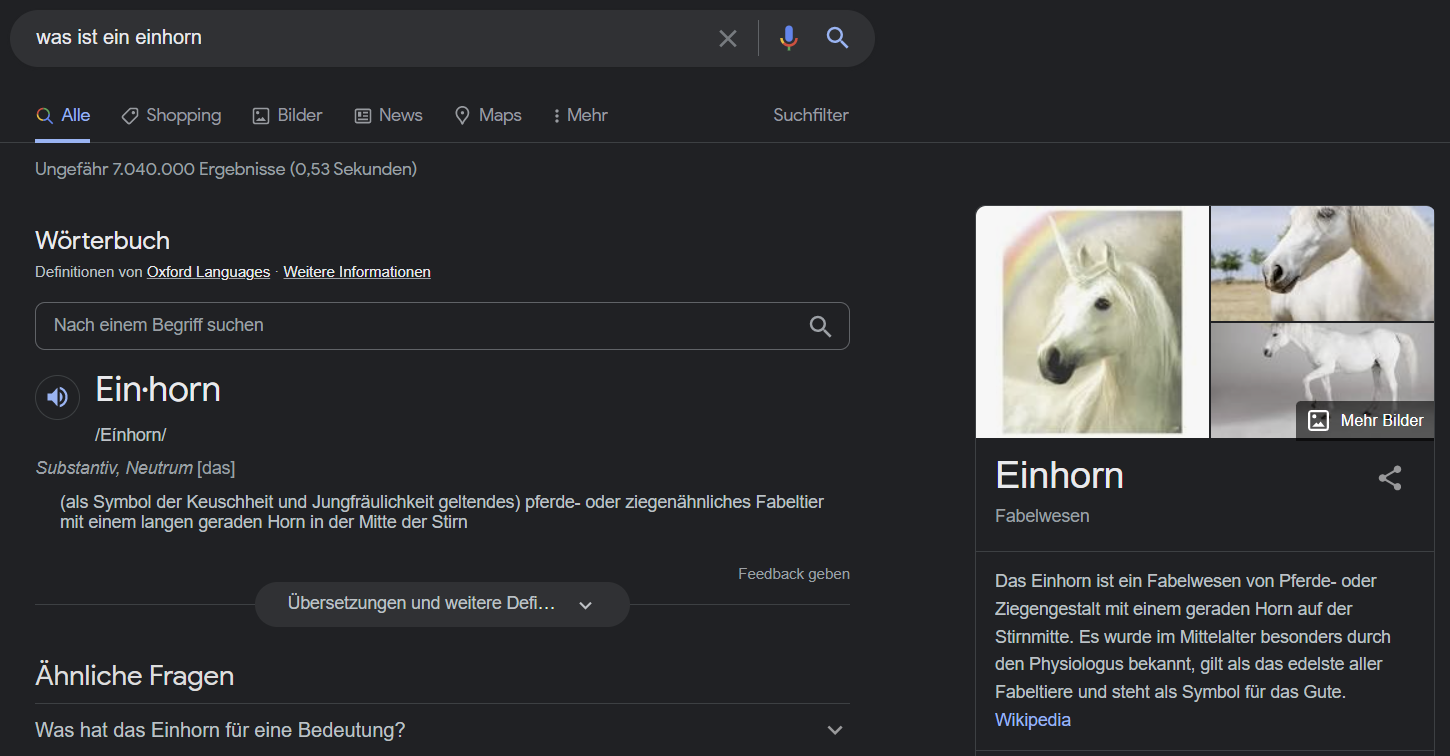
\includegraphics[width=80mm]{images/screenshot_googleQue}
    \caption{Suchergebnis Google}
    \label{fig:screenshotGoogleQue}
\end{figure}
\begin{figure}[h]
    \centering
    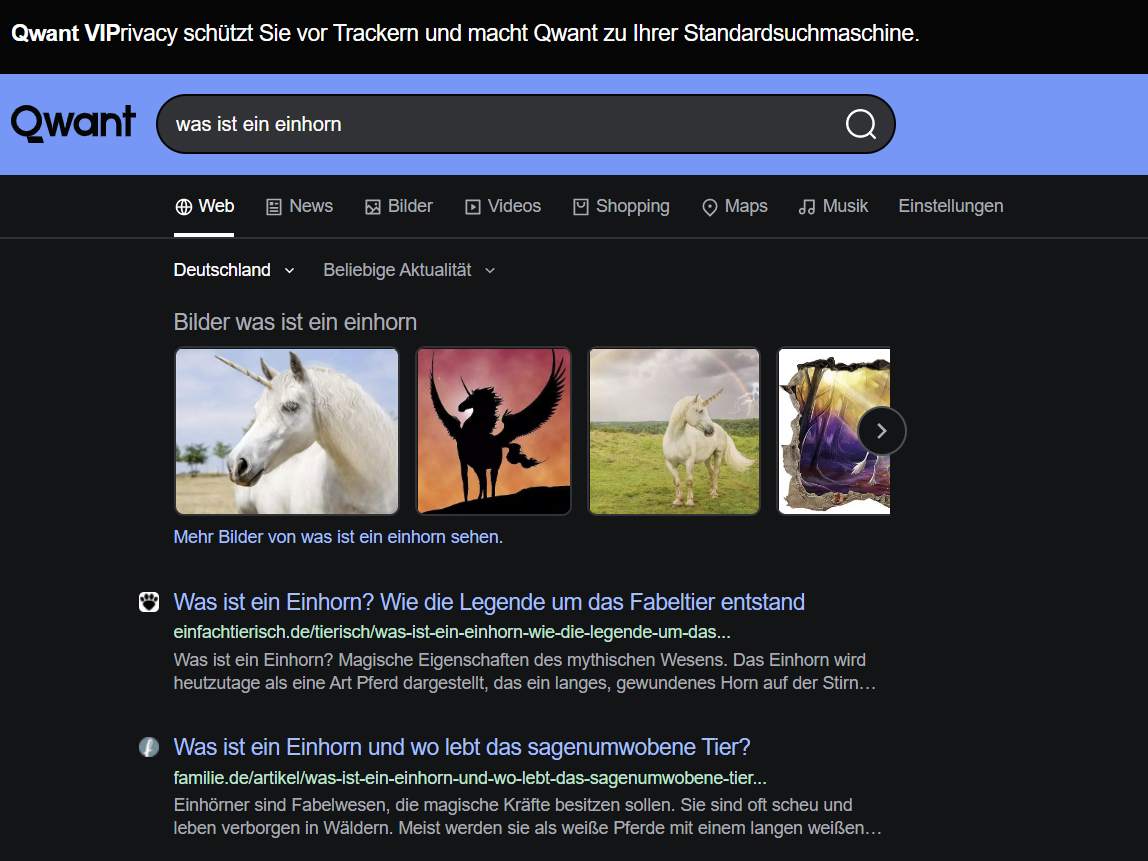
\includegraphics[width=80mm]{images/screenshot_qwantQue}
    \caption{Suchergebnis Qwant}
    \label{fig:screenshotQwantQue}
\end{figure}
Wie man in den angeführten Screenshots sieht, gibt Google direkt die Informationen aus, wo man zum Beispiel bei Qwant zuerst eine Webseite aufrufen muss.
Heute erwarten wir möglichst schnell an die Information zu kommen, worauf sich Google schon angepasst hat.
    \chapter{Fazit}\label{ch:fazit2}

Google, der \gqq{big-player} unter den Suchmaschinen, der mit über 90 Prozent den Markt dominiert,
wird das wohl auch noch eine Weile tun, denn dass der Gigant innerhalb kurzer Zeit zurückgedrängt oder gar abgelöst wird ist bei den aktuellen Nutzerzahlen eher unwahrscheinlich.
Trotzdem gibt es einige Konkurrenten wie Qwant auf dem Markt, die vermutlich nicht zu unterschätzen sind.
Gerade durch einzelne Aspekte, wie Datenschutz, die schon länger kritisch betrachtet werden bei den Branchengiganten wie Google,
können Start-ups wie Qwant sich aus der Menge heben und dem Nutzer eine gute Alternative bieten.
Klar ist, dass es eine ganze Weile, vielleicht eine ganz Generation brauchen wird um einen Giganten wie Google abzulösen,
gerade weil Google es über Jahre hinweg erfolgreich geschafft hat seine Nutzer an sich zu binden.
Letztlich hängt es wohl hauptsächlich von der Entwicklung einzelner Suchmaschinen in der Zukunft ab und wie gut diese sich an den sich ständig weiterentwickelnden Technikmarkt anpassen können,
aber Qwant erfreut sich schon jetzt an steigender Popularität und User sind begeistert von den Aspekten, die ihnen Google nicht bieten kann,
weshalb weiterer Erfolg von kleineren Suchmaschinen und eine Durchmischung des Marktes nicht ausgeschlossen sind.

    %%%%%%%%%%%%%%%%%%%%%%% Literaturverzeichnis %%%%%%%%%%%%%%%%%%%%%%%
    \printbibliography
\addcontentsline{toc}{section}{Literatur}
\newpage


    %%%%%%%%%%%%%%%%%%%%%%%%%%%%%% Anhang %%%%%%%%%%%%%%%%%%%%%%%%%%%%%%
    \renewcommand{\thetable}{\Alph{section}.\arabic{table}}
    \renewcommand{\thefigure}{\Alph{section}.\arabic{figure}}
    \renewcommand{\thelstlisting}{\Alph{section}.\arabic{lstlisting}}
    \pagenumbering{Alph}

    \begin{appendix}
  \section{Anhang}

  \begin{figure}[h]
    \centering
    \fbox{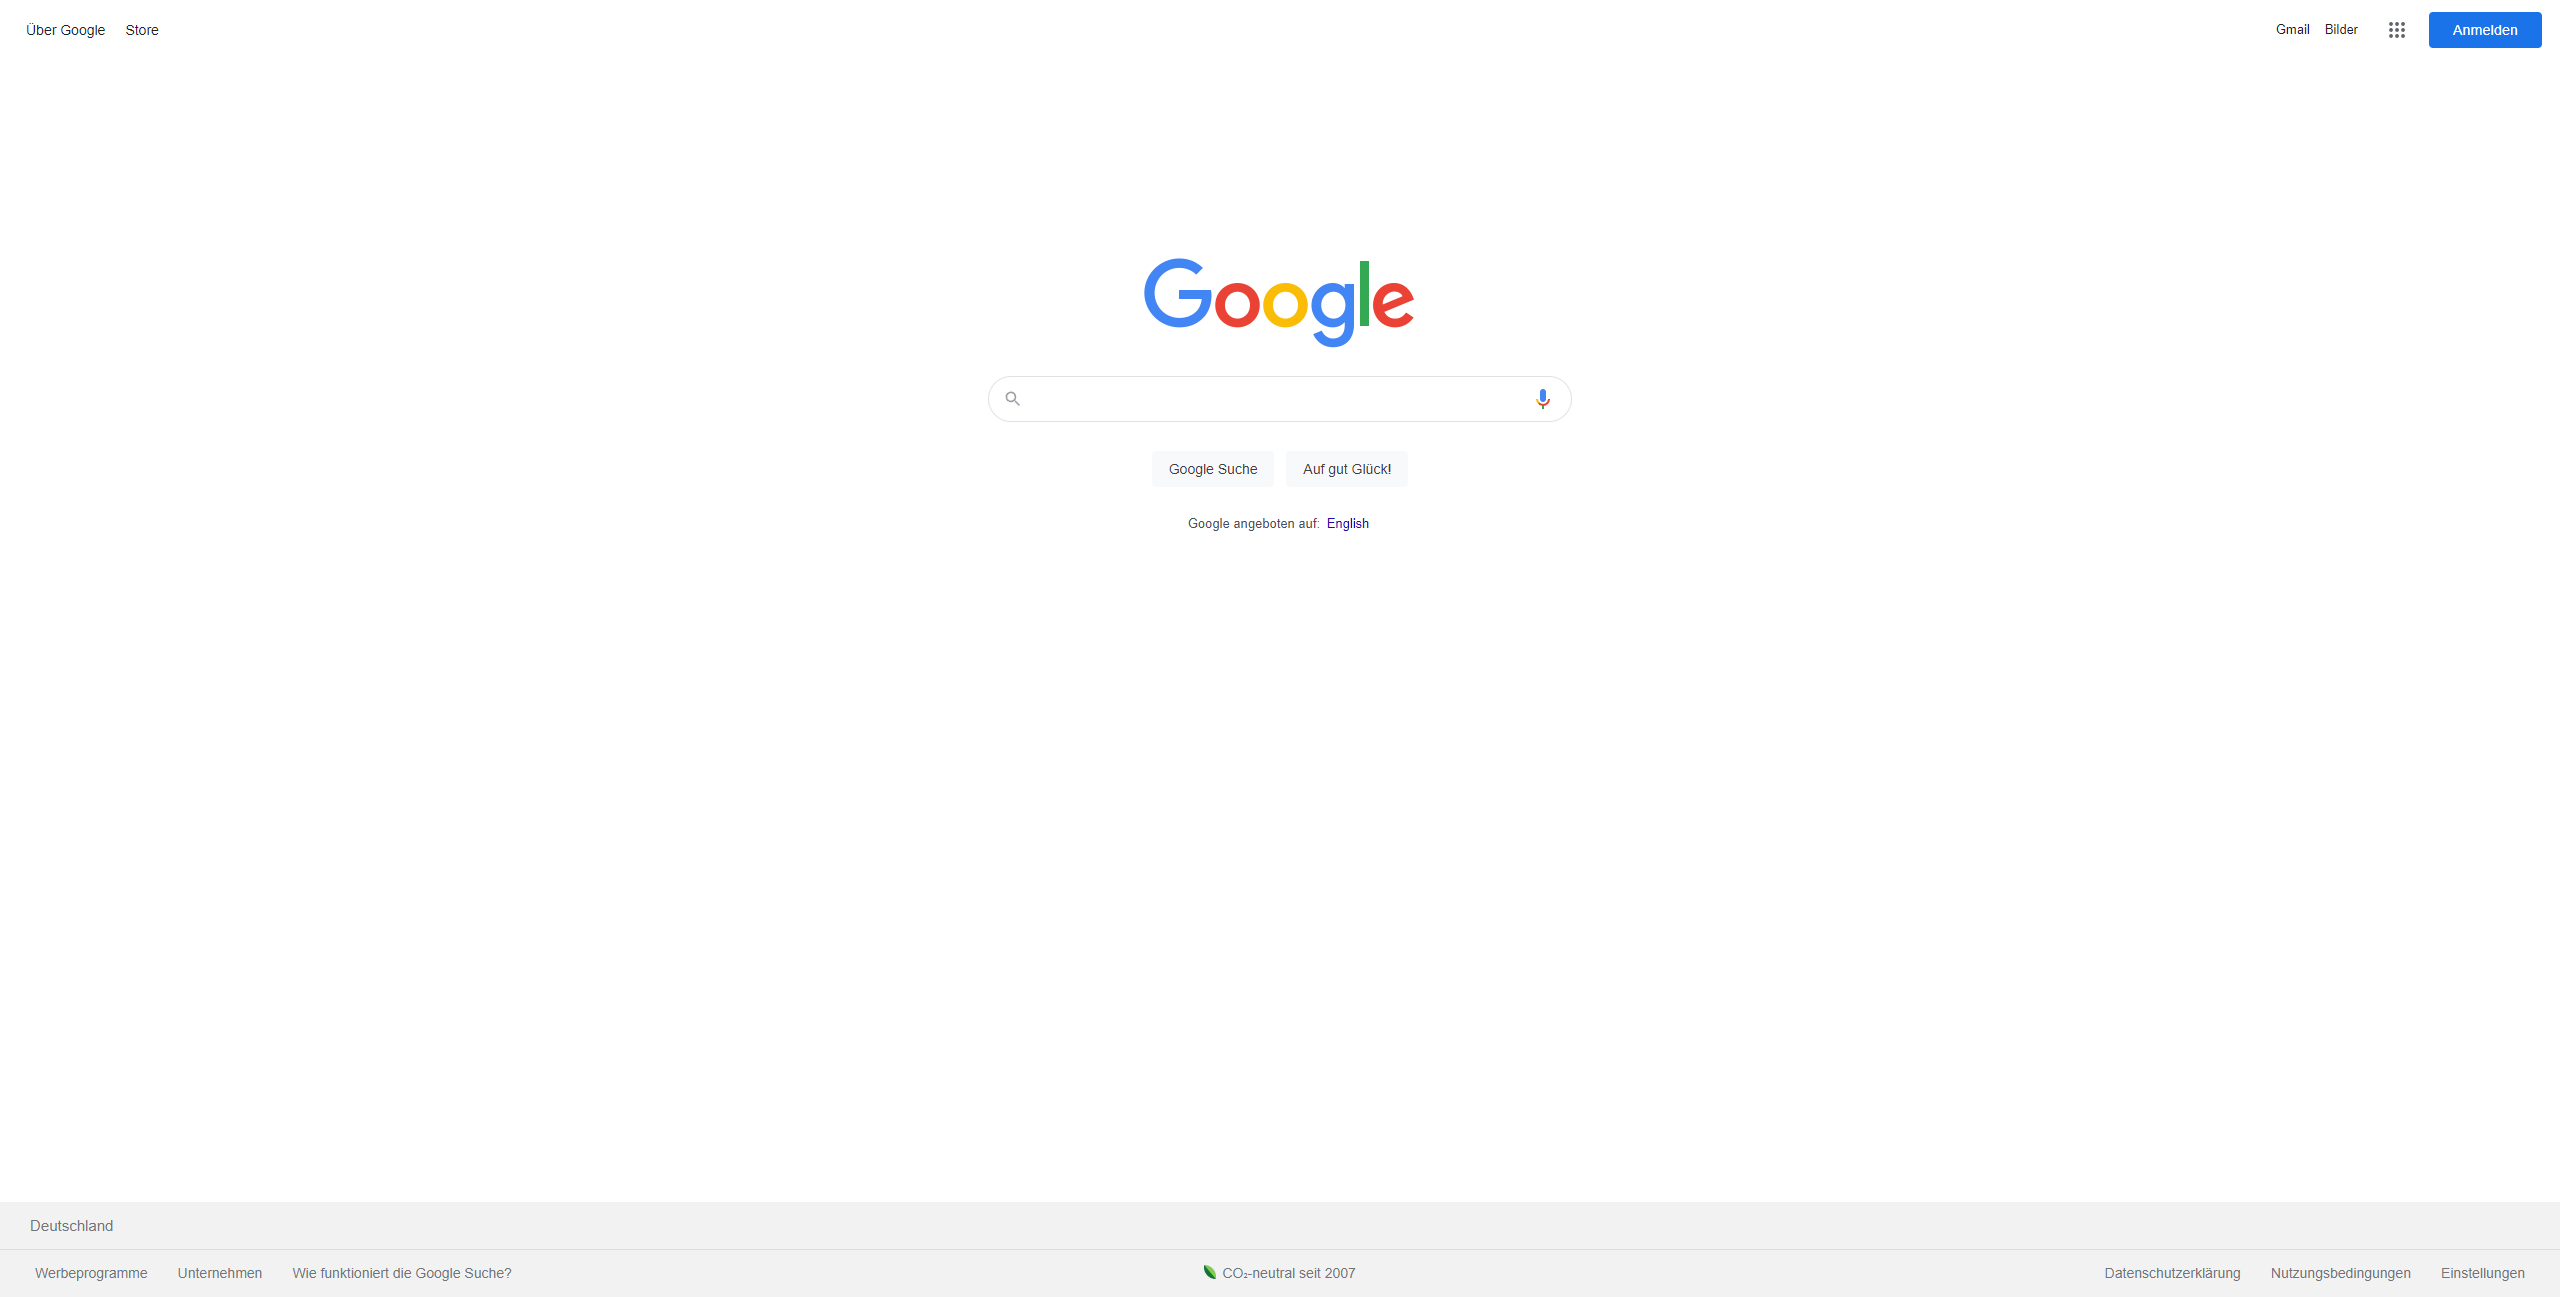
\includegraphics[height=0.3\textheight]{google_home}}\caption{Google Home}\label{fig:google_home}
  \end{figure}
  \begin{figure}[h]
    \centering
    \fbox{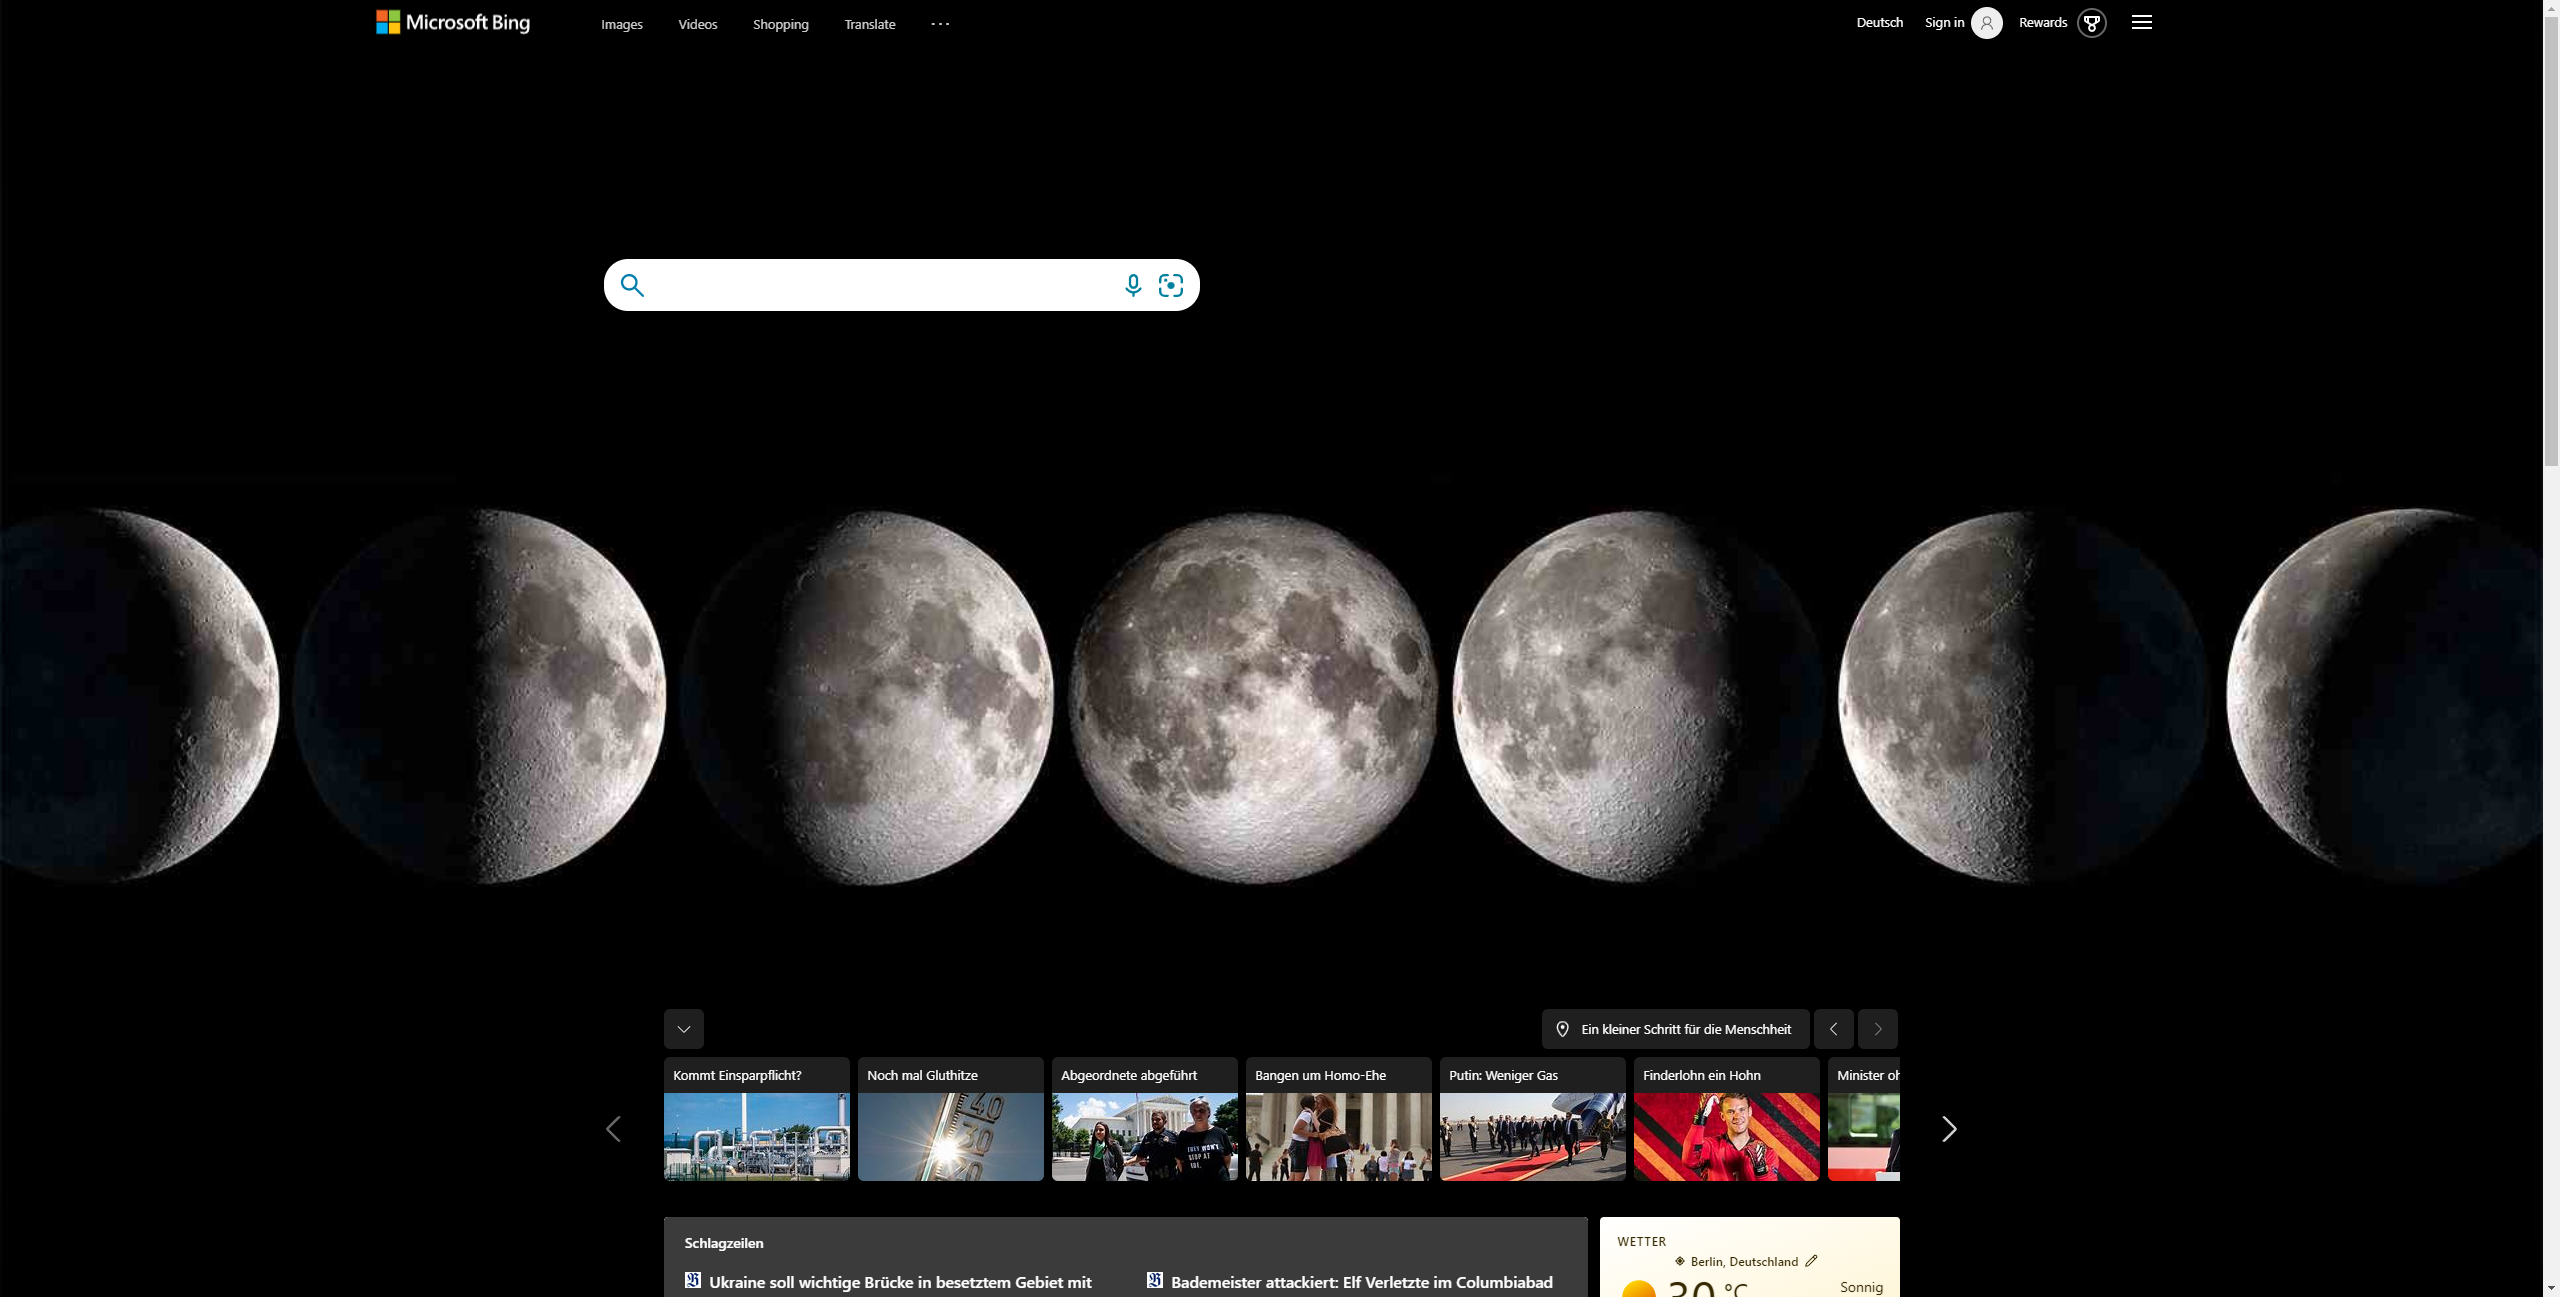
\includegraphics[height=0.3\textheight]{bing_home}}\caption{Bing Home}\label{fig:bing_home}
  \end{figure}
  \begin{figure}[h]
    \centering
    \fbox{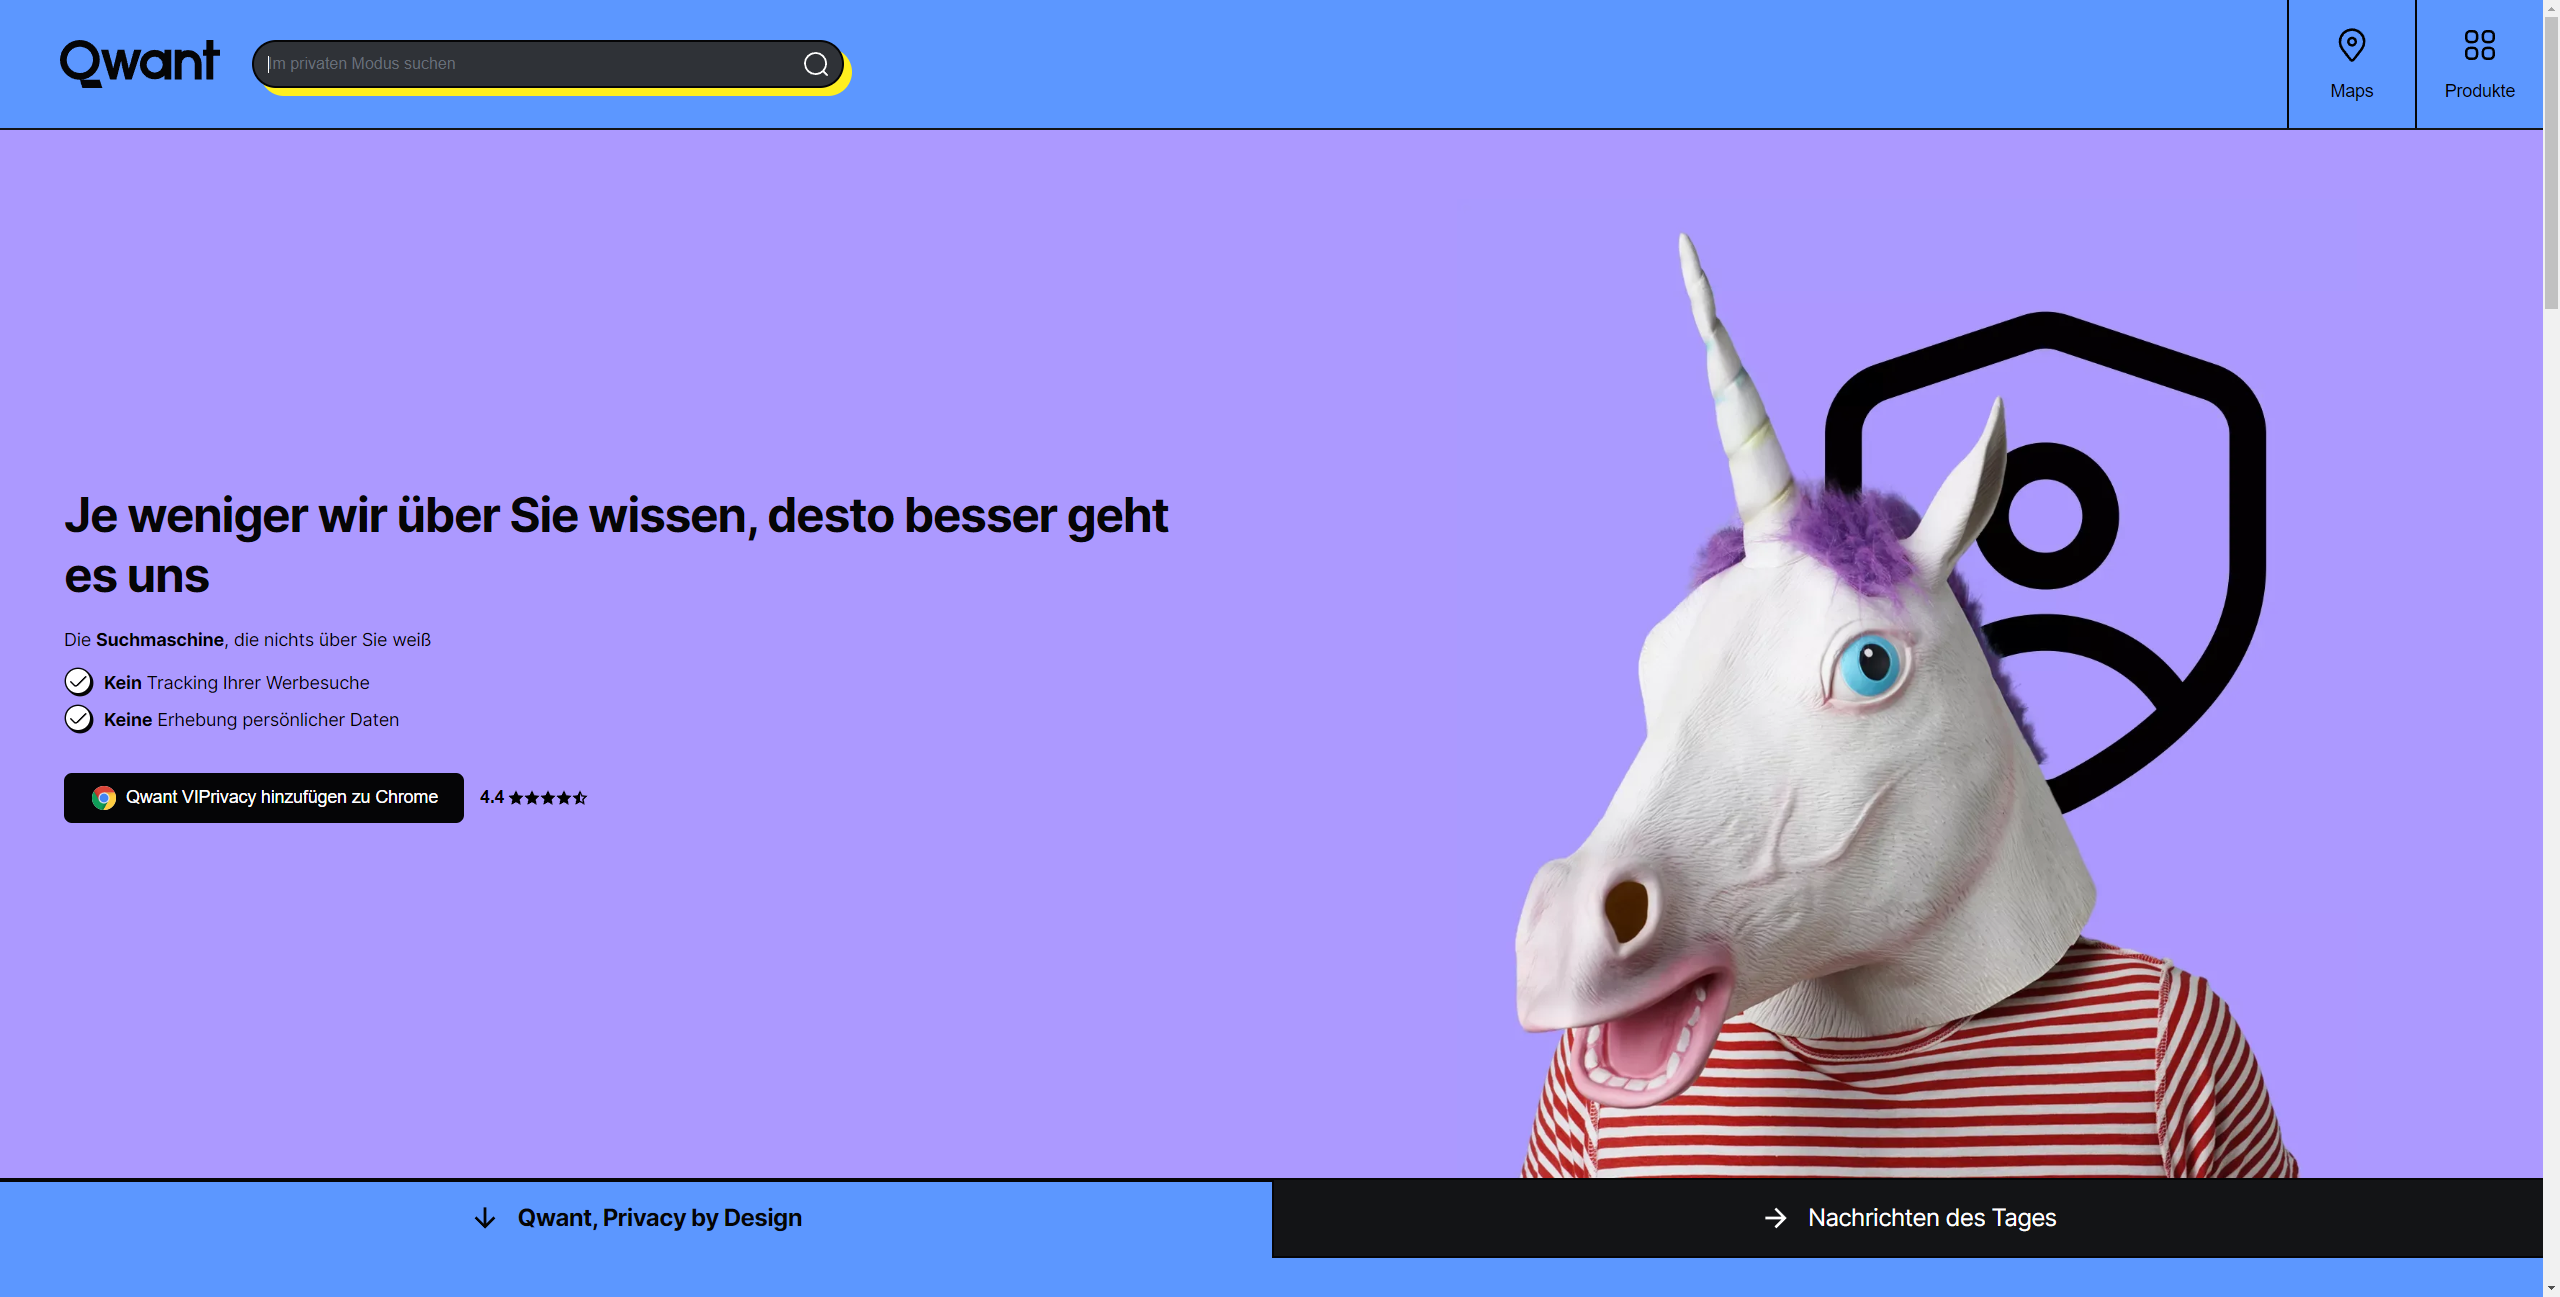
\includegraphics[height=0.3\textheight]{qwant_home}}\caption{Qwant Home}\label{fig:qwant_home}
  \end{figure}
\end{appendix}
\end{document}